\documentclass[]{elsarticle} %review=doublespace preprint=single 5p=2 column
%%% Begin My package additions %%%%%%%%%%%%%%%%%%%
\usepackage[hyphens]{url}

  \journal{WG-EMM 2021} % Sets Journal name


\usepackage{lineno} % add
\providecommand{\tightlist}{%
  \setlength{\itemsep}{0pt}\setlength{\parskip}{0pt}}

\usepackage{graphicx}
\usepackage{booktabs} % book-quality tables
%%%%%%%%%%%%%%%% end my additions to header

\usepackage[T1]{fontenc}
\usepackage{lmodern}
\usepackage{amssymb,amsmath}
\usepackage{ifxetex,ifluatex}
\usepackage{fixltx2e} % provides \textsubscript
% use upquote if available, for straight quotes in verbatim environments
\IfFileExists{upquote.sty}{\usepackage{upquote}}{}
\ifnum 0\ifxetex 1\fi\ifluatex 1\fi=0 % if pdftex
  \usepackage[utf8]{inputenc}
\else % if luatex or xelatex
  \usepackage{fontspec}
  \ifxetex
    \usepackage{xltxtra,xunicode}
  \fi
  \defaultfontfeatures{Mapping=tex-text,Scale=MatchLowercase}
  \newcommand{\euro}{€}
\fi
% use microtype if available
\IfFileExists{microtype.sty}{\usepackage{microtype}}{}
\usepackage[margin=3cm]{geometry}
\bibliographystyle{elsarticle-harv}
\usepackage{longtable}
\ifxetex
  \usepackage[setpagesize=false, % page size defined by xetex
              unicode=false, % unicode breaks when used with xetex
              xetex]{hyperref}
\else
  \usepackage[unicode=true]{hyperref}
\fi
\hypersetup{breaklinks=true,
            bookmarks=true,
            pdfauthor={},
            pdftitle={A preliminary evaluation of the evidence supporting fishery-driven localised depletion effects on the performance and demographic trends of pygoscelid penguins in Subarea 48.1},
            colorlinks=false,
            urlcolor=blue,
            linkcolor=magenta,
            pdfborder={0 0 0}}
\urlstyle{same}  % don't use monospace font for urls

\setcounter{secnumdepth}{0}
% Pandoc toggle for numbering sections (defaults to be off)
\setcounter{secnumdepth}{0}

% Pandoc citation processing

% Pandoc header
\usepackage{pdflscape}
\newcommand{\blandscape}{\begin{landscape}}
\newcommand{\elandscape}{\end{landscape}}
\usepackage{float} \floatplacement{figure}{H} 
\newcommand{\beginsupplement}{\setcounter{table}{0}  \renewcommand{\thetable}{S\arabic{table}}     \setcounter{figure}{0} \renewcommand{\thefigure}{S\arabic{figure}}}
\usepackage{booktabs}
\usepackage{longtable}
\usepackage{array}
\usepackage{multirow}
\usepackage{wrapfig}
\usepackage{float}
\usepackage{colortbl}
\usepackage{pdflscape}
\usepackage{tabu}
\usepackage{threeparttable}
\usepackage{threeparttablex}
\usepackage[normalem]{ulem}
\usepackage{makecell}
\usepackage{xcolor}



\begin{document}
\begin{frontmatter}

  \title{A preliminary evaluation of the evidence supporting fishery-driven
localised depletion effects on the performance and demographic trends of
pygoscelid penguins in Subarea 48.1}
    \author[Norwegian Polar Institute]{Andrew Lowther\corref{1}}
   \ead{andrew.lowther@npolar.no} 
    \author[Institute of Marine Research (Tromsø)]{Martin Biuw\corref{2}}
   \ead{martin.biuw@hi.no} 
    \author[Institute of Marine Research (Tromsø)]{Ulf Lindstrøm\corref{2}}
   \ead{ulf.lindstroem@hi.no} 
    \author[Institute of Marine Research (Bergen)]{Bjørn Krafft\corref{2}}
   \ead{bjorn.krafft@hi.no} 
      \address[Norwegian Polar Institute]{Norwegian Polar Institute, Research Department, Fram Centre, Hjalmar
Johansensgata 14, Tromsø, Norway, 9297}
    \address[Institute of Marine Research (Tromsø)]{Institute of Marine Research, Tromsø 9296, Norway}
    \address[Institute of Marine Research (Bergen)]{Institute of Marine Research, Nordnesgaten 50, 5005 Bergen, Norway}
      \cortext[1]{Corresponding Author}
    \cortext[2]{Equal contribution}
  
  \begin{abstract}
  Two independent lines of evidence have been presented to the working
  groups and SC-CAMLR that claim to demonstrate that fishery-driven
  localised depletion of krill around pygoscelid penguin colonies has had
  a deleterious effect on their performance traits and demographic trends,
  that are equivalent to the impacts of climate variation. One study
  utilises 30 years of penguin foraging and reproductive performance
  measurements collected at two colonies in the South Shetland Islands
  while the other uses demographic rate changes derived from a
  comprehensive dataset of penguin population count data across Subarea
  48.1 matched against acoustic measurements of krill biomass and krill
  catches at the gSSMU scale (Watters et al., 2020). The second uses
  estimated population trajectories across a wide range of penguin
  breeding colonies alongisde krill catches within 30km (Krüger et al.,
  2021). Both studies then explore the synergistic relationships to
  measurements of broad-scale climactic variation (El Nino Southern
  Oscillation; ENSO, and the Southern Annular Mode; SAM). Herein we
  provide a preliminary assessment of the efficacy of both approaches in
  drawing conclusions, that are now being used at the Commission level, as
  representing sound scientific advice. We demonstrate that several
  underlying assumptions in Watters et al.~2020 are contrary to the
  published scientific literature, and when the model syntax is re-written
  to reflect this, predicted penguin performance against long term
  expected means are substantially different to those presented to CCAMLR.
  The analysis provided by Krüger et al. (2021) is less sophisticated,
  however given the details provided we were unable to recreate the
  initial results and could not test the sensitivity of the model to some
  of the assumptions made. We do, however, point to areas in which we have
  concerns, and would welcome collaboration in order to address these.
  Overall while our preliminary assessment focuses on potential issues,
  future work will centre on considering competitive interactions both at
  appropriate time and space scales between the fishery as well as between
  a range of krill dependent predators beyond just pygoscelid penguins.
  \end{abstract}
  
 \end{frontmatter}

\hypertarget{introduction}{%
\section{Introduction}\label{introduction}}

Concerns over the potential impact of localised depletion of krill
through concentrated fishing effort on krill-dependent predators has
been a topic of debate within SC-CAMLR and its Working Groups for many
years. Recently, two studies have been presented that suggest that local
harvesting rates can impact predator performance to the same degree as
poor environmental conditions (Watters et al., 2020) and when poor
climactic conditions are coupled to locally high harvest rates the
synergistic impacts on predators are evident (Krüger et al., 2021).

While both studies attempt to tackle the same overall problem, they do
so using very different methodologies. Watters et al. (2020) exploit a
considerable dataset; a substantial multi-species time series of a large
number of penguin performance indices (including those collected under
CEMP) collected over three decades at two sites (Cape Shireff on
Livingstone Island and Copacabana on King George Island, South Shetland
Islands; Figure 1) and over a decade of summer acoustic krill surveys
that cover the at-sea distributions of Chinstrap, gentoo and Adélie
penguins. Drawing in monthly krill catch statistics from the C1 Catch
and Effort dataset and climactic data (Oceanic Niño Index; ONI), the
authors use a hierarchical analysis of variance approach to estimate the
variance in performance indices as a function of Local Krill Biomass
(LKB), Local Harvesting Rates (LHR; the ratio of krill catch to LKB) and
ONI. In contrast, Krüger et al. (2021) utilise a broader range of
penguin colonies across the same three species throughout the Antarctic
Peninsula area, in combination with their respective abundance survey
estimates (number of occupied nests) from an open-source database
(www.penguinmap.org). The authors calculate population trends for
appropriate sites, and using the CCAMLR C1 Catch and Effort data to
extract annual catch values within a 30km radius of each colony.
Finally, Krüger et al. (2021) use the sign of the difference in the
number of nests between annual surveys as a response in a binomial
generalised linear mixed effects model using the accumulated annual
catch and the mean wintertime Southern Annular Mode (SAM) to determine
the relative contributions of each predictor and their interactive
effects on population abundance trends. Both studies draw similar
conclusions; that local harvesting levels of krill impact predators, and
the degree of impact can either be similar to that of poor environmental
conditions or have a synergistic impact when high local harvesting
coincides with poor conditions.

These conclusions have been propagated into Commission documentation
supporting the reformulation of the D1MPA proposal (CCAMLR-39/BG/02) as
well as into Commission discussions (CCAMLR-39, Para 5.48 \& Para 5.51).
However, while the two studies have moved from Working Papers of EMM
into the realm of the peer-reviewed literature, there are some areas of
concern regarding the structuring of these studies that we think deserve
attention. Some of these concerns are unique to each study while others
are common across both, and we structure our paper accordingly. Firstly,
we review Watters et al. (2020) and Krüger et al. (2021) through the
lens of some of the ecological assumptions made versus the available
evidence pertaining to them. Within the constraints of the data and
analytical methods that are available from the studies, we also quantify
how rationalising these assumptions to the evidence available impacts on
the conclusions drawn. We then highlight some overarching concerns
applicable to both papers.

\hypertarget{watters2020-wg-emm-201911}{%
\section{Watters et al. (2020) / WG-EMM
2019/11}\label{watters2020-wg-emm-201911}}

A key goal for the paper is to highlight the mismatch between the areal
scales of fisheries management and ecological interactions between
fishing extractions and dependent predators. To do this, the authors
create two strata aligned with groups of SSMU (gSSMU); gSSMU \#1
including those SSMU inside the Bransfield Strait (APBSE and APBSW) and
gSSMU \#2 incorporating SSMU north of the South Shetlands, including
Elephant Island (APDPE, APDPW and APEI) represented in Figure 1. These
gSSMU cover \(15,500nm^2\) and \(20,600nm^2\), respectively, and are
used to characterise both krill biomass and harvesting rates that are
``local'' to the penguin colonies for which performance data are used.
The reasoning behind scaling to gSSMU are linked to the foraging
behaviour of the penguins for which performance data area available
i.e.~breeding, adult pygoscelids. The authors cite Hinke et al. (2017)
as the evidence supporting usage of the two gSSMU as appropriate strata.

Pygoscelid penguins exhibit staggered breeding, with Adélies commencing
first, followed by Chinstraps then Gentoos (Black, 2016). Adélie
penguins are the first to fledge their chicks and thus cease to be
centrally foraging, typically departing mid-February for their moulting
grounds on the sea ice. Chinstrap penguins depart for a pre-moult
foraging trip towards the end of February and return to land in order to
moult, before departing again for their overwinter trip (Hinke et al.,
2015, 2019)(Figure 2). Conversely, Gentoo penguins appear to remain in
close proximity to their breeding colonies overwinter (Korczak-Abshire
et al., 2021).

We use the Argos-CLS PTT telemetry data provided by the supporting
studies to characterise the actual at-sea habitat used, in the context
of the relative stage of breeding for each species (though we also
recommend Warwick-Evans et al. (2018) and Lowther et al.~(this meeting)
amongst other work, for further quantification of foraging behaviour of
breeding penguins in this area). For each species, we refrain from
undertaking extensive state-space modelling of location errors and
merely exclude locations with a ``Z'' error class, accepting the
remaining locations had varying degrees of uncertainty around them, then
calculated the 99\% Minimum Convex Polygon (home range) using the R
package \emph{``adehabitatHR''}and their associated areas in \(nm^2\).
For Chinstrap penguins at Cape Shireff, this equated to a home range
area of \textasciitilde{}\(4,782nm^2\), or only 23\% of the gSSMU to
which their performance metrics are indexed against (Watters et al.,
2020). For the same species at Copacabana the 99\% MCP home range is
2,905\(nm^2\), or \textasciitilde19\% of gSSMU 1 in the Bransfield
Strait. Similarly for Adélie penguins, the breeding foraging range
occupied 1,139\(nm^2\) or only \textasciitilde7\% of the area of gSSMU
\#1. After breeding, available overwinter PTT telemetry and light
geolocating data on chinstrap and Adélie penguins suggests a wide
dispersal westwards into the Pacific sector of the Southern Ocean, and
eastwards into the Weddell Sea and Atlantic sectors, with a relatively
small proportion of chinstraps from the study sites remaining within
500km of their breeding colonies (Hinke et al., 2019). Yet despite the
evidence supporting widescale post-breeding migration of both Adélie and
Chinstrap penguins, the model used by Watters et al. (2020) constrains
both species from Copacabana to gSSMU 1 and Chinstraps from Cape Shireff
to gSSMU 2 over winter (Supplementary Material 1 \& 2, code lines 258 to
259). This has the effect of constraining the variability in performance
indices from these species to LHR, LKB and ONI over winter in areas
where the species has a demonstrated tendency to migrate away from. This
is particularly important given that the fishery can now be
characterised with a late autumn/early winter start which places a
seasonal element on LHR towards increased values in the winter (Figure
4).

Our preliminary review thus far raises two areas of concern. Firstly,
that the scales at which ``local'' predictors are summarised are in some
cases five times larger than the habitat exploited by the penguins
monitored. Local Harvest Rate is a function of the catch and its
distribution; we demonstrate catch variability across breeding seasons
within the original gSSMU, using available C1 Catch and Effort data
during the austral summer period, relevant to the breeding season and
thus centrally foraging Adélie and Chinstrap penguins between 2009 and
2018 for Subarea 48.1 (Supplementary Figure 1).

Secondly, that the known overwinter migratory behaviour of Adélie and
Chinstrap penguins are poorly reflected in the model formulation. To
demonstrate the impact that these ecological assumptions have on the
model output, we rerun the model of Watters et al. (2020) with modified
code. To avoid an overly burdensome paper, we shortly summarise those
code changes here, and if requested during the meeting we are happy to
include the rmarkdown version of this paper with the modified code in
place, or submit the modifications to the meeting in some other format.

We also note an additional coding error that may influence how the
original, unmodified results are interpreted. In summarising the model
outputs into boxplots, the code relating to developing Figure 2
(Supplementary Material 1, lines 661-665) seemingly classifies the
``Worst Case'' with ``neutral'' ONI (\({-0.5}\) \(^{\circ}\)C
\textless{} ONI \textless{} 0.5 \(^{\circ}\)C; LKB \textgreater{} 1 Mt;
and LHR \(\geqslant\) 0.1) using Parameter set 36 from the output
dataframe, which actually reflects a ``warm'' ONI component
(\textgreater{} 0.5 \(^{\circ}\)C; LKB \textgreater{} 1 Mt; and LHR
\(\geqslant\) 0.1). Yet the discussion in Watters et al. (2020) suggests
that the likelihood of their ``Worst Case'' includes future warming.

We agree that any ``Worst Case'' should reflect ENSO conditions into the
future under a warming climate. However, climate change is likely to
increase ENSO in amplitude - both El Niño (ONI ``warm'') and La Niña
(ONI ``cold'') (Capotondi et al., 2015). How this increasing amplitude
can be integrated appropriately into the presented modelling framework
to match with long-term predicted mean performance of predators has not
been explored yet. As such, and for the sake of comparison with the
original study, we maintain the authors designation of ONI ``neutral''
when rendering the ``Worst Case'' boxplots, though caution that this is
unlikely to be a realistic expectation.\\
\newline \emph{Modifications}\\
1. We scale the gSSMU LKB to the SSMU that the summer tracking data
indicate penguins occupied. To do this, we calculate the area (\(nm^2\))
of the SSMU for which the predator occupies and the gSSMU to which it is
assigned, then create a scaling ratio. For example, we scale LKB for
Cape Shireff Chinstrap penguins solely to ADPDW (Figure 1) by
multiplying the gSSMU LKB by the areal ratio of ADPDW/gSSMU \#2. We then
select the corresponding SSMU catch values provided in Watters et al.
(2020) to estimate SSMU-scale LHR. We also caution that while
considering the gSSMU scale of harvesting as inappropriate for ``local''
effects, even the SSMU-scale catch levels likely do not reflect
pressures at scales relevant to breeding penguins (Supplementary Figure
1). 2. We remove Adélie and Chinstrap penguins from the model
formulation over winter; that is, we attribute each species as ``NA''
during winter (to account for dsipersal after breeding), thus removing
them from association with any gSSMU.\\
3. The authors place LKB/LHR values in March into the ``summer'' period.
However fishing effort over the period that performance indices are
available is not uniform over the thirty year period, with catch over
the preceding decade showing a nonlinear increase from the middle of
March and three years where catch rates increased rapidly from the
beginning of the month (Figure 4). Given the highly variable rates of
catch throughout the study period, we run scenarios that classify March
as either summer or winter to reflect the linkage between March and the
breeding state of penguins i.e.~Adélie and Chinstrap penguins have
either migrated out of the area or have ceased to be centrally foraging
species by March.

Thus we reformulate the underlying assumptions above into a new model
construct, in which performance indices from all three species during
the summer are included, but Adélie and Chinstrap penguins cease to be
centrally foraging species after breeding and migrate out of the area.
The performance indices are matched in space and time but using SSMU
level estimates of LKB and LHR. We re-run this reformulation using the
original analysis of variance model framework that includes imputed
values for LKB in years where survey data are missing. We further
consider two alternatives for considering March, either in a) summer or
b) winter.

We present the outputs both in the same boxplot format as Figure 2 in
the original manuscript, and as individual cases grouped and
colour-coded as ONI ``warm'' (\(\geqslant\) 0.5; red), ONI ``neutral''
(-0.5 \textless{} ONI \textgreater{} +0.5; white) and ONI ``cold''
(\textless{} -0.5; blue). We also recreate the original marginal
probabilities in Table 1 of Watters et al. (2020), and two additional
tables in the same format with the probabilities extracted from our
reformulated model, the difference between the latter two tables
reflecting whether March is in summer or winter.\\
\newline   \emph{Results}\\
From the original Watters et al. (2020) model, the probability that the
Worst Case would cause penguin performance indices to drop below their
long-term mean was 77\%, while relative to the Best Case there was a
93\% probability that penguin performance would decline as a response to
high LHR. Similarly, there was a 99\% probability that high LHR and LKB
under neutral ONI (``Worst Case'', though see above for comments on
this) would drive penguin peformance to fall below its long term mean
(Table 1).

Our reformulation paints a very different picture, and while we refrain
from providing an exhaustive in-text comparison, we highlight a few
examples here. Comparing the original model outputs with ours, relative
to the Best Case, the probability of negative impacts to penguins due to
high LHR dropped precipitously from \(\geqslant\) 93\% to 37\% (Table
3). In other words, considering the migration of penguins in accordance
with their known ecology, the relative probability of negative impact of
LHR drops from a near-certainty to 1-in-3 (Table 2 and 3). Given the
temporal separation between fishing and penguin breeding over the
preceding decade, our results are unsurprising.

The probability that the effects of warm or neutral ONI would be more
detrimental to penguin performance were greater than for the Worst Case
(Table 2 and 3). When we consider the marginal effects of neutral ONI
and high LHR, the probabilities that the former would negatively impact
penguin performance below the long-term mean was x4 greater than the
impact of high LHR (Table 2 and 3). Looking at the case-by-case and
selected plots in Figure 3 the overwhelming dominace of the ONI state
can clearly be seen. La Niña (``cold'' ONI) conditions resulted in
predictive probabilities of performance that were equal to, or
surpassing, those of the Best Case irrespective of increased LKB or LHR.
Even more bizarrely, an increase in LHR to even high levels has a lower
probability of decreasing penguin performance than the Best Case (Table
2 and 3). It is important to note that, overall our intention is not to
suggest that increased fishing is beneficial; merely that when the model
is reconditioned on ecological knowledge, the outputs in its current
formulation should be treated with caution.

Thus while the authors contend that they have little doubt that penguins
are responding to both the environment and fishing, we contend that they
are reacting to the environment, and the scales at which their model
incorporates fishing bear no relevance to the scales at which penguins
exploit. The authors of the original model also identifying an
insensitivity of penguin performance to marginal changes in LKB and as
reflecting previous failed attempts to parameterise functional responses
of penguins - we fully agree as our reanalysis draws similar conclusions
of insensitivity, but we propose that even the SSMU scale is
inappropriate for matching food availability and harvesting pressure to
predator performance (Figure X).

\hypertarget{kruger2021-wg-emm-201910}{%
\section{Krüger et al. (2021) / WG-EMM
2019/10}\label{kruger2021-wg-emm-201910}}

The key objective of the paper by Krüger et al. (2021) is to examine the
potential synergistic effects of climate change and increased fishing
activity in recent decades on the breeding performance of Chinstrap and
gentoo penguins. The authors make the implicit assumption that there has
been a general decrease in krill density in response to climate change,
although this is still a topic of debate and is not supported by recent
large-scale surveys in the Scotia Sea (SG-ASAM 2019/08 Rev.1).

\textbf{\emph{Perhaps describe the model already here, to set the scene
for the data input issues? - YEP}}

To address this topic, the authors use data on the number of occupied
nests (breeding pairs) counted at a large number of sites throughout the
Antarctic Peninsula between 1980 and 2017. These data are available from
the Mapping Application for Penguin Populations and Projected Dynamics
(MAPPPD) data archive (www.penguinmap.com; Humphries et al. (2017)).
Krüger et al. (2021) include count data on occupied nests based on
surveys carried out in November or December, reflecting the early
breeding season. They further subset the data to include only colonies
for which at least 2 survey estimates are available throughout the
38-year period under consideration (i.e.~1980-2017). These data are
provided in the supplementary materials for the paper. Based on the raw
counts, they calculate an index of temporal variation in population
growth rate using: \[\lambda_{std}=((n_b/n_a)/years_{b-a}-1\] where
\(n\) is the number of breeding pairs counted in Nov-Dec of a given
year, \(b\) and the number of breeding pairs counted in the nearest
previous year \(a\) in which a Nov-Dec survey was conducted, divided by
the interval between surveys (i.e.~\(b-a\)). While this index may be a
robust index of population change, the authors then convert
\(\lambda_{std}\) into a binary index, \(bin\lambda_{std}\) that takes
the value 1 for negative growth and 0 for positive growth. The rationale
is that this value can be interpreted as the probability of population
decline (irrespective of its magnitude) in response to catch and
environmental change. However by only taking the sign of the change and
creating a binary response the authors completely ignores the magnitude
of the absolute or relative this change in population size; that is, a
decline of 1\% or 99\% is considered equivalent in the model.

Another problem with this index is the interval between consecutive
surveys. Based on the Krüger et al. (2021) supplementary dataset,
intervals between surveys exceeding one year are relatively common
(intervals \textgreater1 year: 26\% for Chinstraps and 47\% for Gentoos;
intervals \textgreater2 years: 15\% for Chinstraps and 14\% for Gentoos,
Table 1). As we describe below, these larger intervals may represent a
temporal mismatch problem, given the fact that response variables only
represent conditions within the one year prior to the breeding season.

As in the case of Watters et al. (2020), Krüger et al. (2021) also use
CCAMLR C1 Catch and Effort data from the krill fishery to estimate
fishing pressure, but in this case only hauls within a 30km radius are
considered for each specific colony. This selection is based previous
observations that foraging of pygoscelid penguins is more probable
within 30 km of the colonies during the breeding season (Warwick-Evans
et al., 2018). While they initially summarise these data within distinct
time periods (reflecting different important stages of the penguin
annual cycle), these are only used for illustrative purposes (Fig 3 in
Krüger et al., 2021). When modelling the effect of fisheries on
population response, the authors then use accumulated annual catches
within these 30km areas, making the assumption that the number of
breeding penguins counted in a given survey is affected by resource
availability in the immediate vicinity of their specific breeding
colonies during the non-breeding period in winter. While this might be
valid for gentoo penguins which appear to remain close to the breeding
colonies also outside the breeding season (Korczak-Abshire et al.,
2021), it is questionable how appropriate this is for Chinstraps that
disperse much more widely during winter (see above section and
references therein). This spatio-temporal mismatch problem is further
exacerbated in cases where intervals between consecutive breeding
population surveys exceed one year (Table 4).

The authors use monthly data on the Southern Annular Mode (SAM) index to
represent environmental variability (Doddridge and Marshall, 2017; Kwok
and Comiso, 2002). Based on an observed 0-3 month lagged correlation
between SAM and relevant local climate variables (fractional sea ice
cover, open water sensible heat flux and sea level air pressure), the
authors exclude SAM values for months coinciding with the breeding
season. As discussed in the review of Watters et al. (2020) above, the
climactic conditions over the WAP are a function primarily of the
Amundsen Sea Low and its interactions with both ENSO and SAM as well as
the bathymetry of the local areas. There is a rich scientific literature
addressing climate-driven hydrographic variability in the WAP , none of
which is considered in this paper.

To test statistically the effects of local fishing pressure and
environmental conditions on penguin breeding performance, Krüger et al.
(2021) fit a binomial Generalized Linear Mixed Effects model of the
form: \[bin\lambda_{std}=catch_y*SAM+(1|colony\text{ }ID)\] where
\(catch_y\) is the accumulated krill catch within 30km of each colony
during the year immediately leading up to the second survey in an
interval (i.e.~equivalent to \(year_b\) in the population growth rate
equation above), SAM is the SAM index during the winter prior to the
same survey (i.e.~temporally overlapping with most of the catch data
accumulation period) while the term in brackets indicate a random
intercept effect on colony. Fundamentally, unlike in the case of Watters
et al. (2020), scripts are not provided for the analyses done by Krüger
et al. (2021), and therefore we have not been able to recreate the
original dataset, their analyses or test various aspects of data input,
underlying assumptions and alternative model formulations. Over 50\% of
the gentoo penguin colonies examined have never been exposed to positive
catch rates within the 30km radius. As such, our concerns lie in the
underlying assumptions, and we would welcome the opportunity to
collaborate openly on a) recreating these analyses and b) testing their
sensitivity to the assumptions made.

\begin{enumerate}
\def\labelenumi{\arabic{enumi}.}
\setcounter{enumi}{2}
\item
  The validity of linear interpolation across multiple years
  (\textgreater1) has not been analysed.
\item
  No consideration of lagged recruitment (fledging to reproductive age)
  nor ability to detect lagged recruitment with irregular surveying
  effort / lack of banding
\end{enumerate}

\textbf{Problem 1: There's clearly some discrepancies in amounts of data
here that we may need to approach the authors about.}

\textbf{Problem 2: How representative is this rate value for a specific
year, in the cases where it has been calcluated as a linear change over
a period of several years between surveys?}

\textbf{Problem 3: Is it appropriate to use annually accumulated catch
as an explanatory variable to explain number of breeding pairs observed
in Nov-Dec?}

\textbf{Problem 4: In the case of gentoos, half of the sites never have
positive catch rates within 30 km, while for chinstraps the situation is
not so bad. How does this explain the model fits and conclusions of
Kruger et al.?}

\textbf{Problem 5: If no other climate variables are included in the
model, does their argument really make sense? Why exclude SAM during the
breeding period?}

\textbf{Problem 6. According to the documentation ,this package only
appears to have the capacity to fit a simple LMME, which does not allow
for a binomial response - SEE ABOVE COMMENT - lmerTest loads in lmer4
which as binomialGLMM capability ?}

\hypertarget{discussion}{%
\section{Discussion}\label{discussion}}

Our preliminary review of the evidence supporting localised effects of
fishing coupled with broad-scale climactic phenomena having an impact on
the vital statistics of pygoscelid penguins (performance and demographic
trends) are based on assumptions that potentially do not reflect current
knowledge of penguin breeding phenology and movement.

Of greatest concern, however, is that the interpretation of model
outputs from both approaches (either from both the original studies or
the modified parameters we describe) are under boundary conditions that
we feel are not appropriate. Both approaches consider only the fishery
and broad-scale climate phenomena as the only two causes of krill
abundance variability at geographic scales relevant to penguins. Neither
study considers, for example, the impact of rebounding baleen whale
populations or migratory male Antarctic fur seals beyond brief
mentioning. HUmpback whales have increased in abundance throughout the
life of the krill fishery, and there are sufficient telemetry and
distance sampling studies in the scientific literature to demonstrate
the degree and significance of spatiotemporal overlap with breeding
penguin populations (see Santora and Veit (2013), Lowther et al. (2020),
Oosthuizen et al., Johannessen et al.~and Lowther et al.~submitted to
this meeting, and Figure 3 as examples). Importantly, the distribution
of these and numerous other unconsidered competitors is not uniform in
either space or time, and their impact on local availability of krill is
likely to be considerable.

Similarly, the utilisation of broad-scale climatological phenomena to
characterise impacts at scales that predators are dependent upon is
problematic. The Amundsen Sea Low (ASL) is the dominant climate feature
for the western Antarctic Peninsula. The El Niño Southern Oscillation
(ENSO) modulates the the ASL, with El Niño (La Niña) shallowing
(deepening) its pressure, causing more northwesterly (southeasterly)
winds and upwelling (restricted influx) of Circumpolar Deep Water onto
the shelf. The Southern Annular Mode also influences the pressure of the
ASL, with the current trend of negative SAM constructively
(destructively) interfering with ASL when in phase with El Niño (La
Niña) events (e.g.~Clem et al. (2016)). The result is a set of
above-surface climate conditions that drive changes in water mass
intrusion that is in turn dependent on \emph{interactions} between two
climate processes. The bathymetry of the Antarctic Peninsula which also
influences the hydrographic conditions is complex (particularly at
scales that are important to centrally-foraging predators such as
penguins) and the structuring of krill aggregations in time and space in
the WAP have been linked to mesoscale circulation processes (Santora et
al., 2012), which are unlikely to be uniformly affected by macroscale
processes.

Our work into the future will progress along three lines, and we welcome
any and all offers of collaboration into this work. Firstly, we will
progress this debate into the scientific literature in order to ensure a
balanced discussion occurs in that forum. Secondly, we will be examining
in further detail some of the additional predictors used and their
efficacy, the modelling frameworks into which they are brought, and how
their incorporation influences the interpretation of the responses.
Finally, we shall also be exploring alternative modelling approaches
that reflect more of the physical and biological complexity of the
system in question. In all cases, our goal is to ensure that the best
available objective scientific evidence is presented to our
environmental managers and, where appropriate, flag that disagreement
exists. Our paper should be viewed in this light to generate
constructive dialogue that addresses our common concern of the potential
for localised fishing to impact dependent aspects of the ecosystem.
\newpage  

\begin{figure}
\includegraphics[width=0.65\linewidth]{./Watters EMM figures/Penguin distributions} \caption{Penguin foraging behaviour during summer breeding, derived from available ARGOS-CLS PTT data presented in Hinke et al. 2017. A) Chinstrap penguins from Cape Shireff (blue) and Copacabana (green) truncated at $10^{th}$ March in line with known phenology (Black 2016; Lowther et al.(this meeting).  Elongated grey track represents a single animal) B) Adélie penguins truncated to the end of January and C) Gentoo penguins until \textasciitilde{}August, representing all available PTT data provided. The SSMU are combined and coloured according to gSSMU (red; gSSMU 2, purple; gSSMU 1) with Chinstrap and Adélie penguin 99\% MCP home ranges occupying between 7-19\% of the gSSMU to which they were assigned.}\label{fig:Penguin distribution plots}
\end{figure}

\begin{figure}
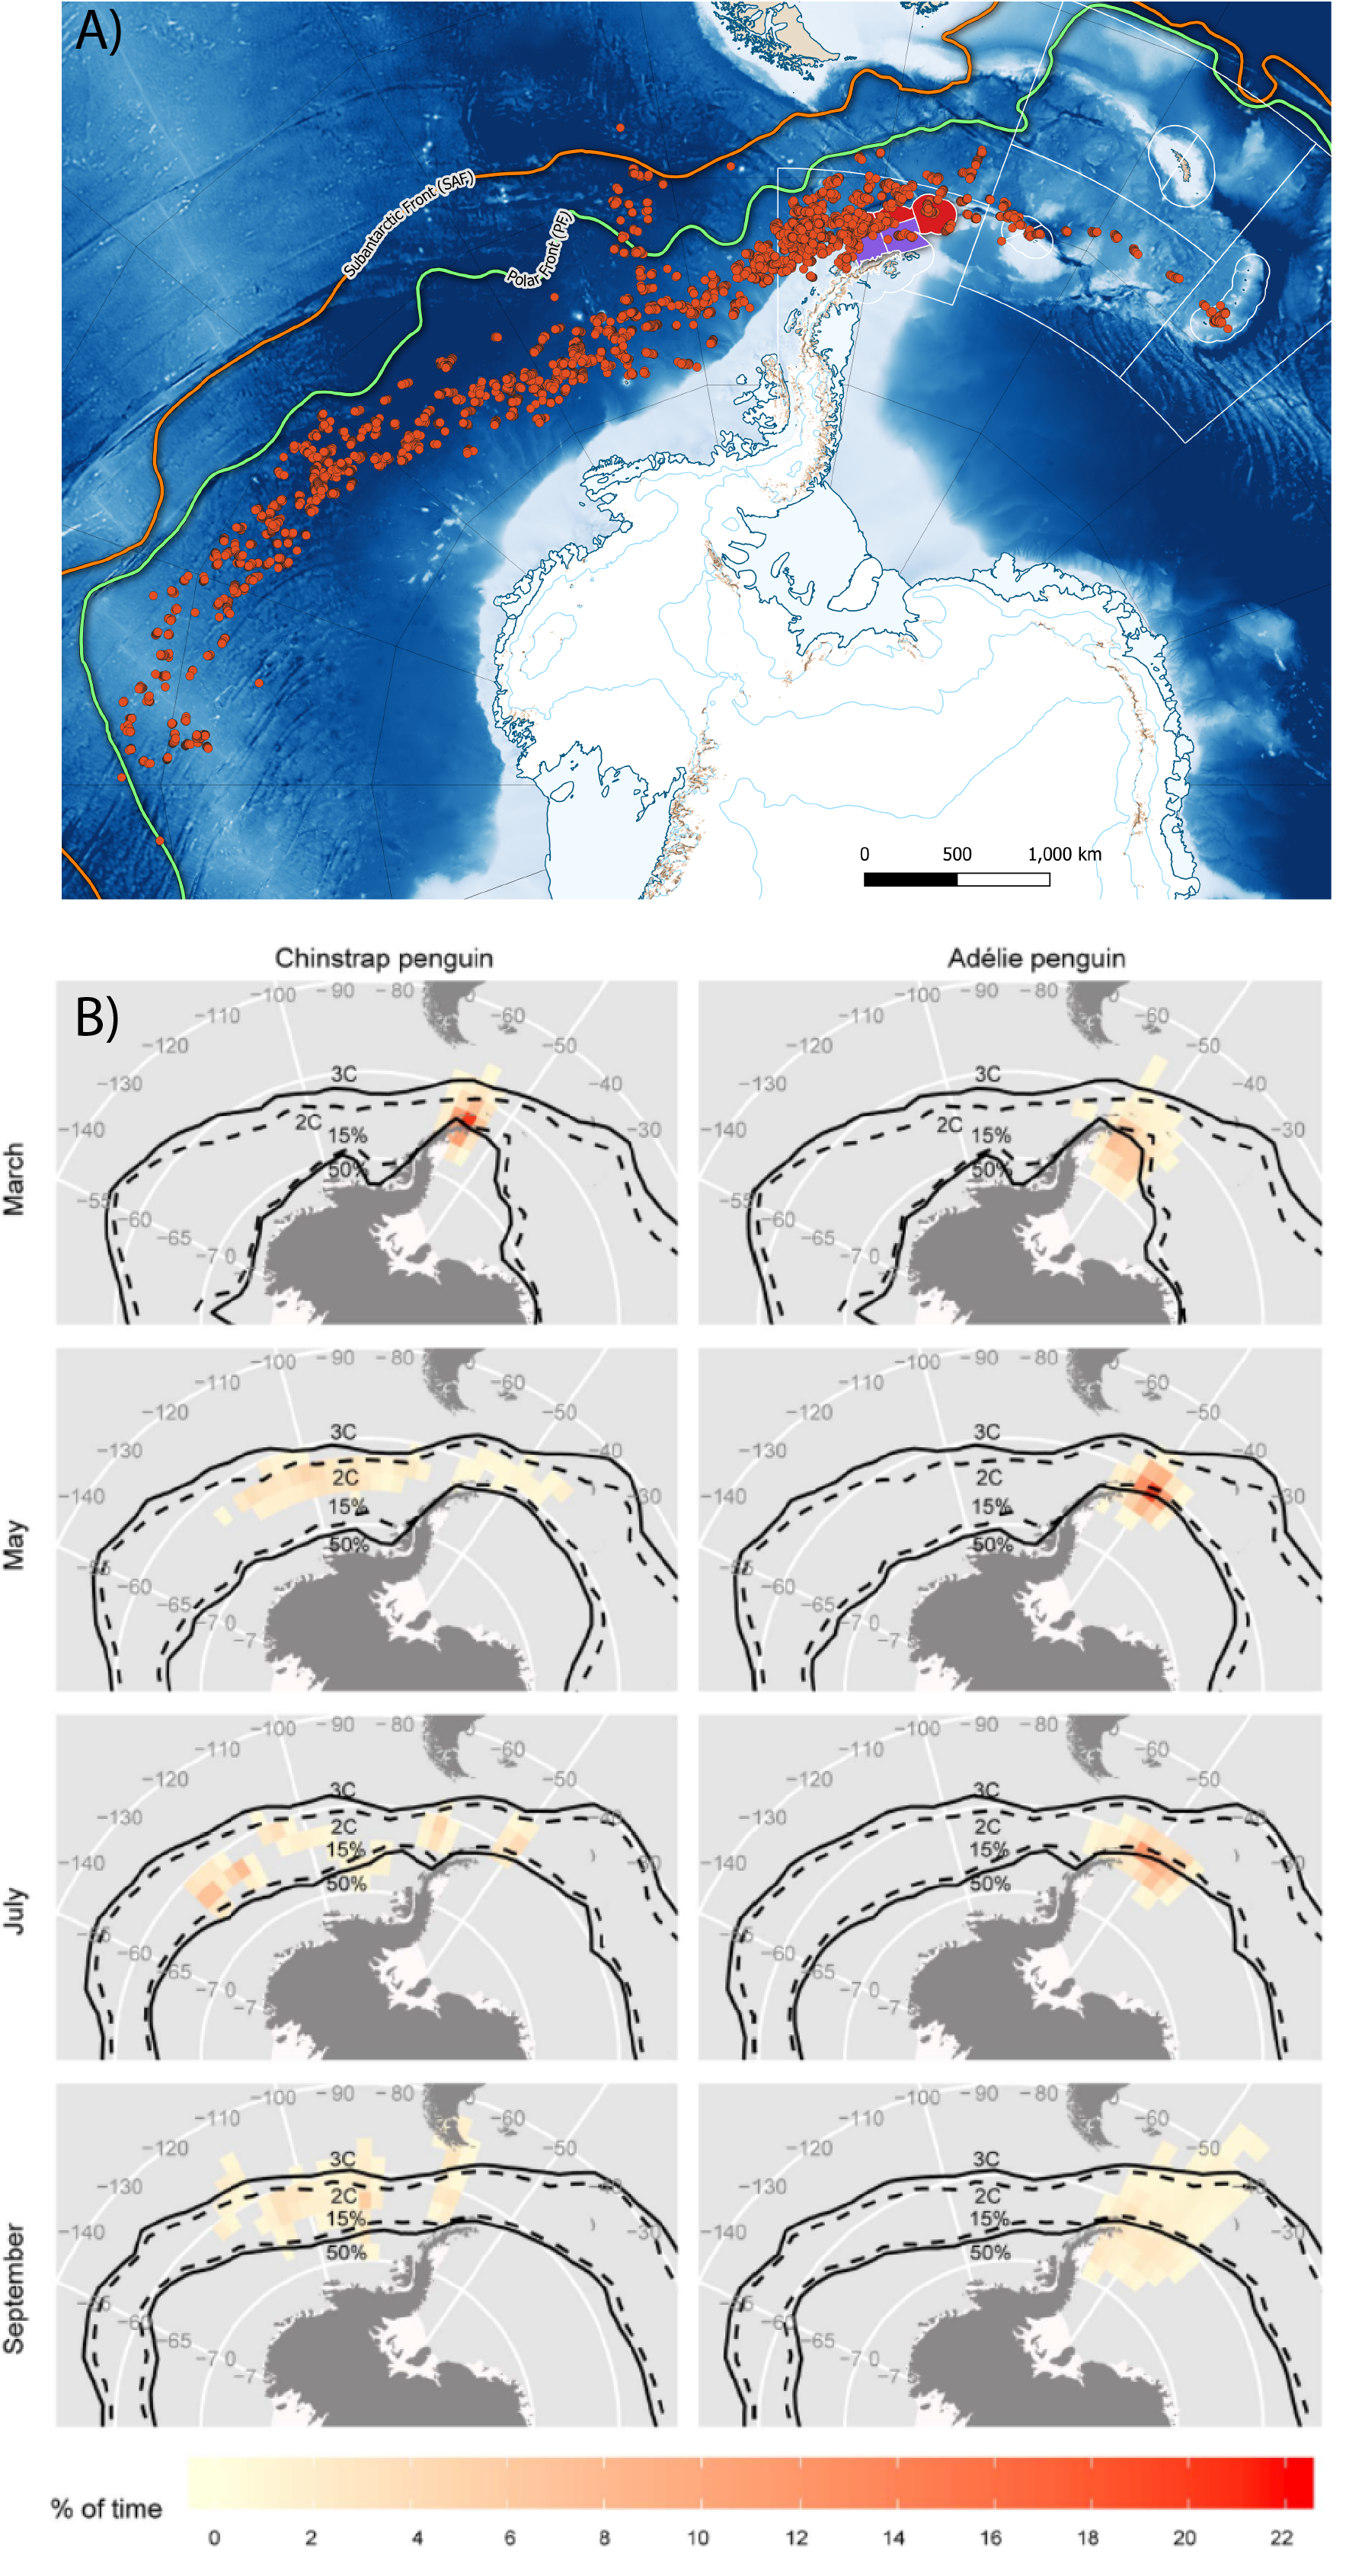
\includegraphics[width=0.75\linewidth]{./Watters EMM figures/Overwinter pengo distributions} \caption{A) Distribution of overwinter movement for Chinstrap penguins, relative to the gSSMU's to which they were attributed, created from telemetry data available in Hinke et al. 2019.  B) Adélie and Chinstrap penguin movement recorded by light geolocators, highlighting the large longitudinal range both species disperse through at the end of breeding (taken from Hinke et al. 2015).  In the original model formulation by Watters et al. 2020, the performance indices for both species are matched to gSSMU-scale estimates of LKB and LHR and macroscale levels of ONI variability.}\label{fig:Overwinter penguin  plots}
\end{figure}

\begin{figure}
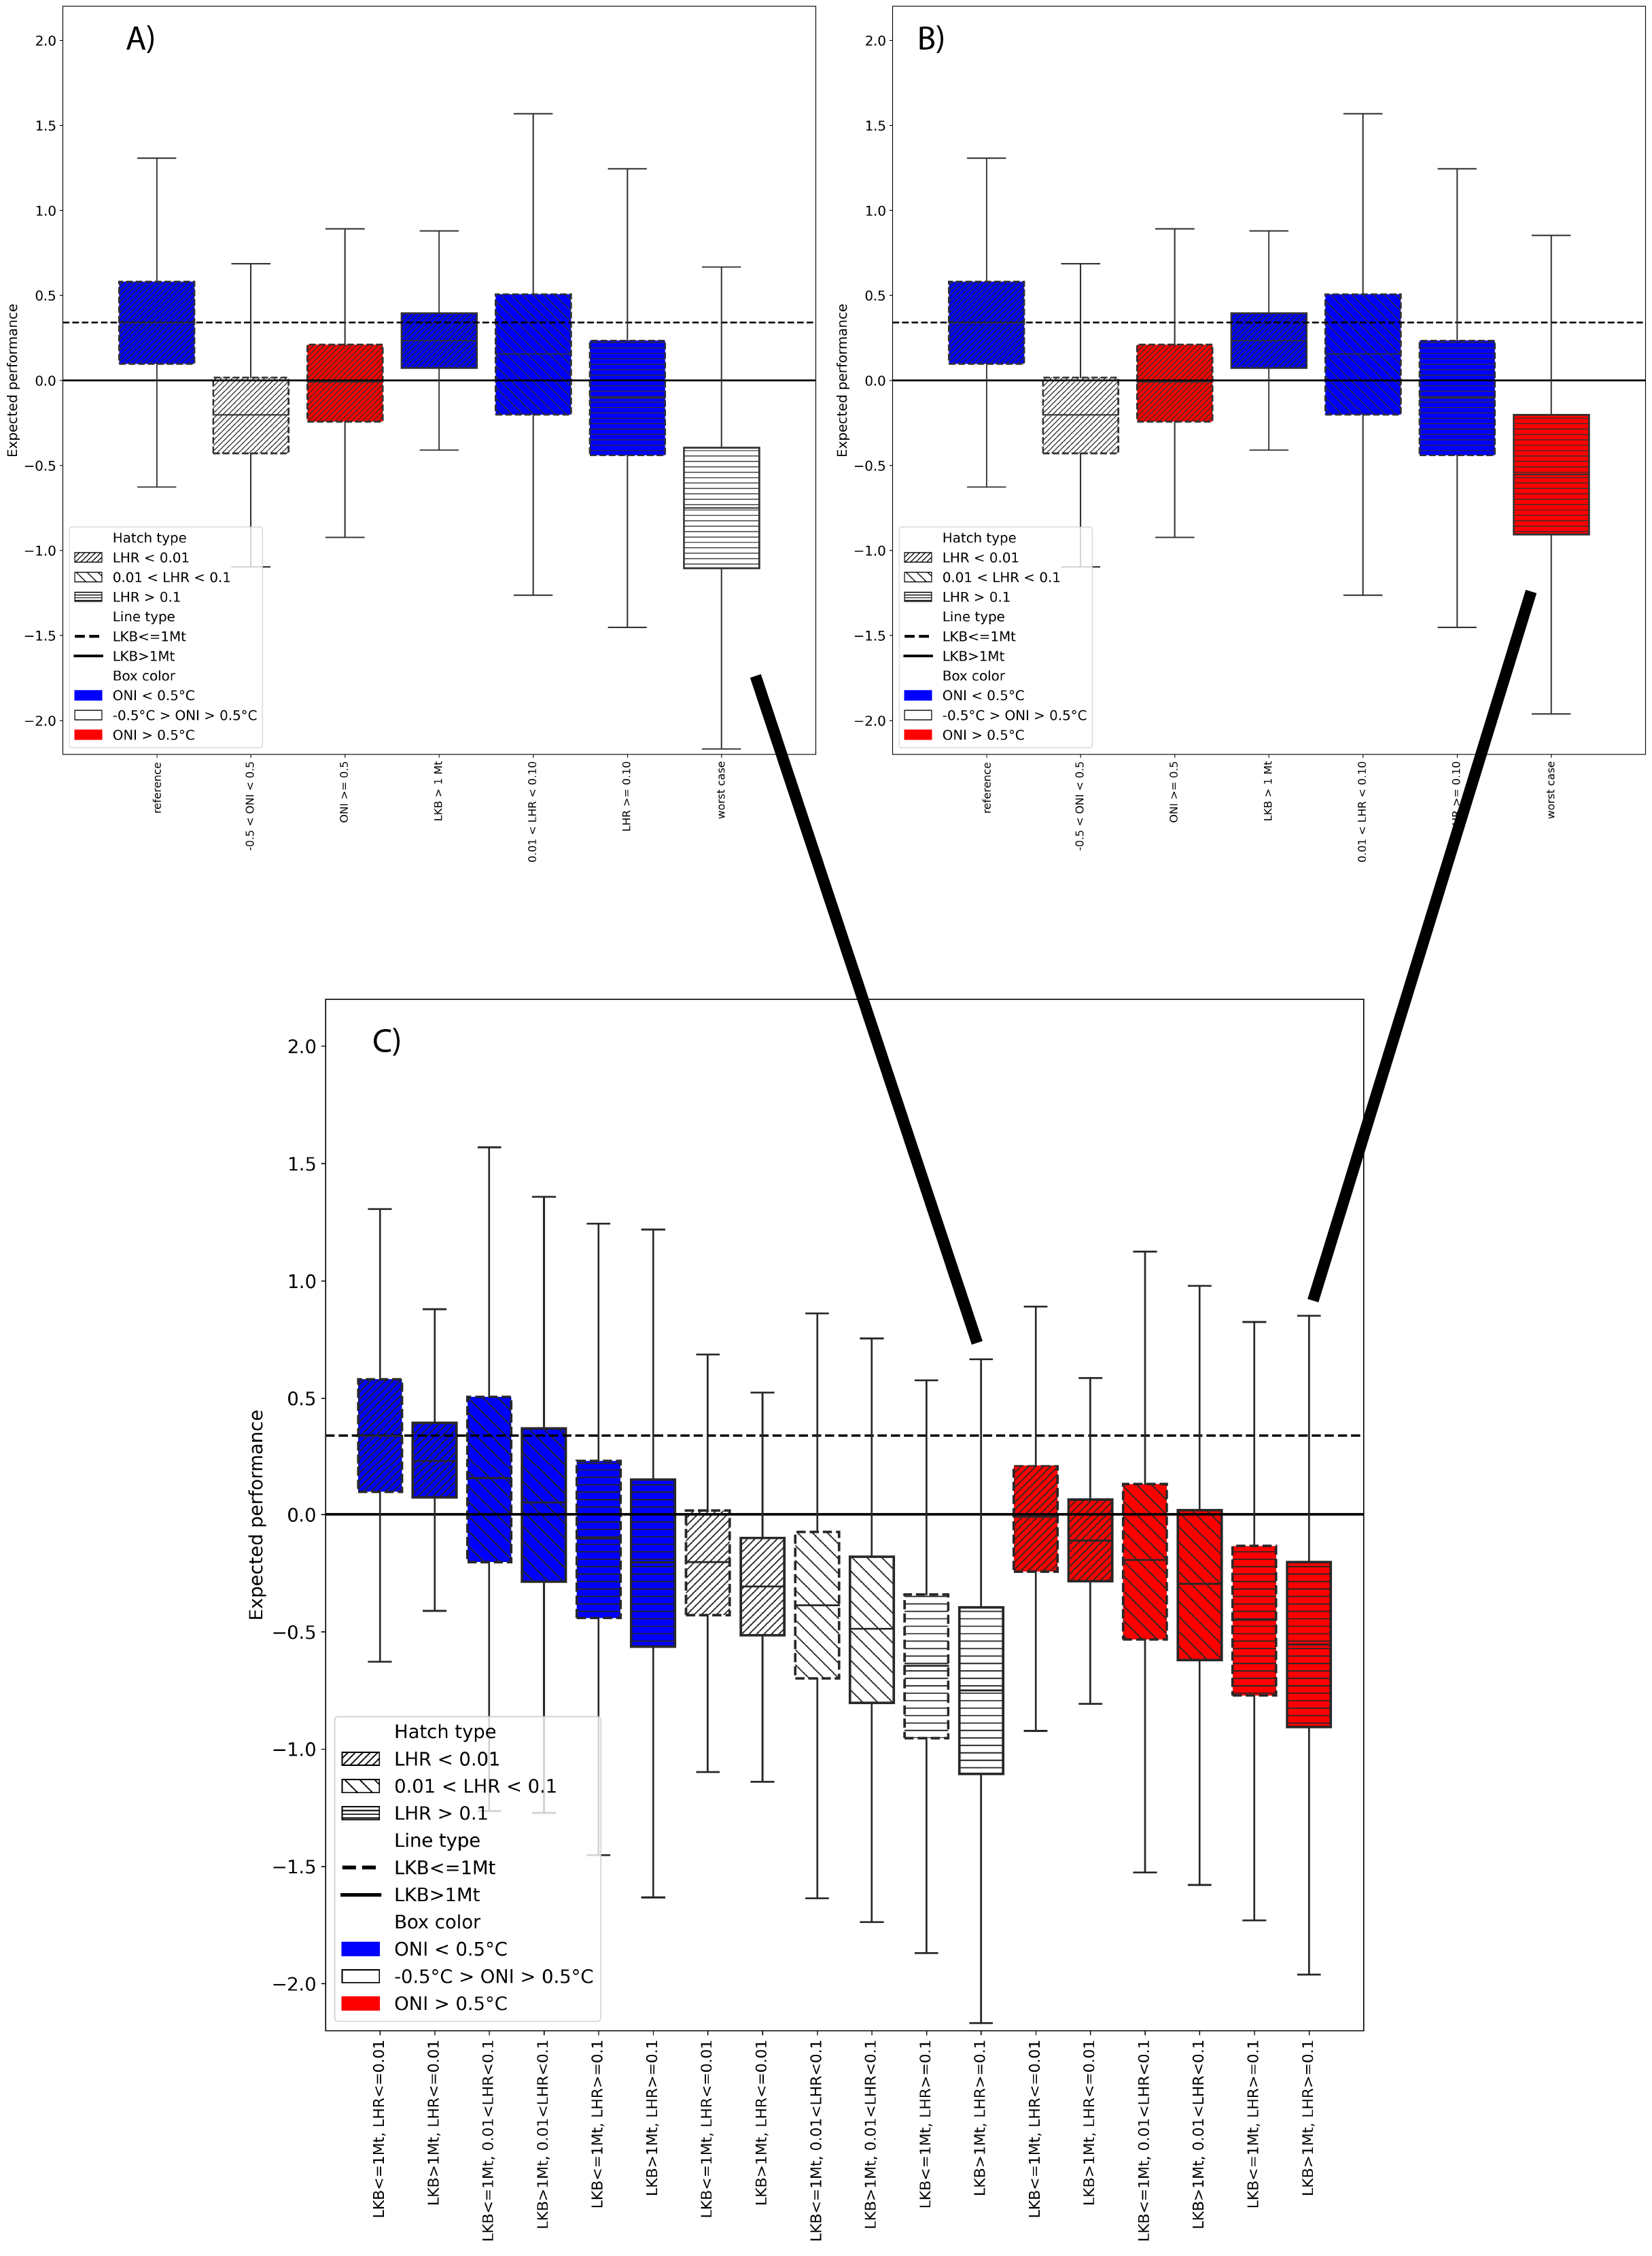
\includegraphics[width=0.75\linewidth]{./Watters EMM figures/Watters original and mistake} \caption{Original Figure 1 plot from Watters et al. 2020 with A) Neutral ONI and B) B) Warm ONI constituting the Worst Case selected.  C) Displays the original case-by-case plots recreated from the paper, with Case 12 representing the intention while data from Case 18 was selected for rendering the boxplot.  Henceforth, to facilitate comparison, we refer to the ONI Neutral plot however we consider this unrealistic if the intention is to portray a Worst Case of a continuing warming climate.}\label{fig:Watters original and mistake}
\end{figure}

\begin{figure}

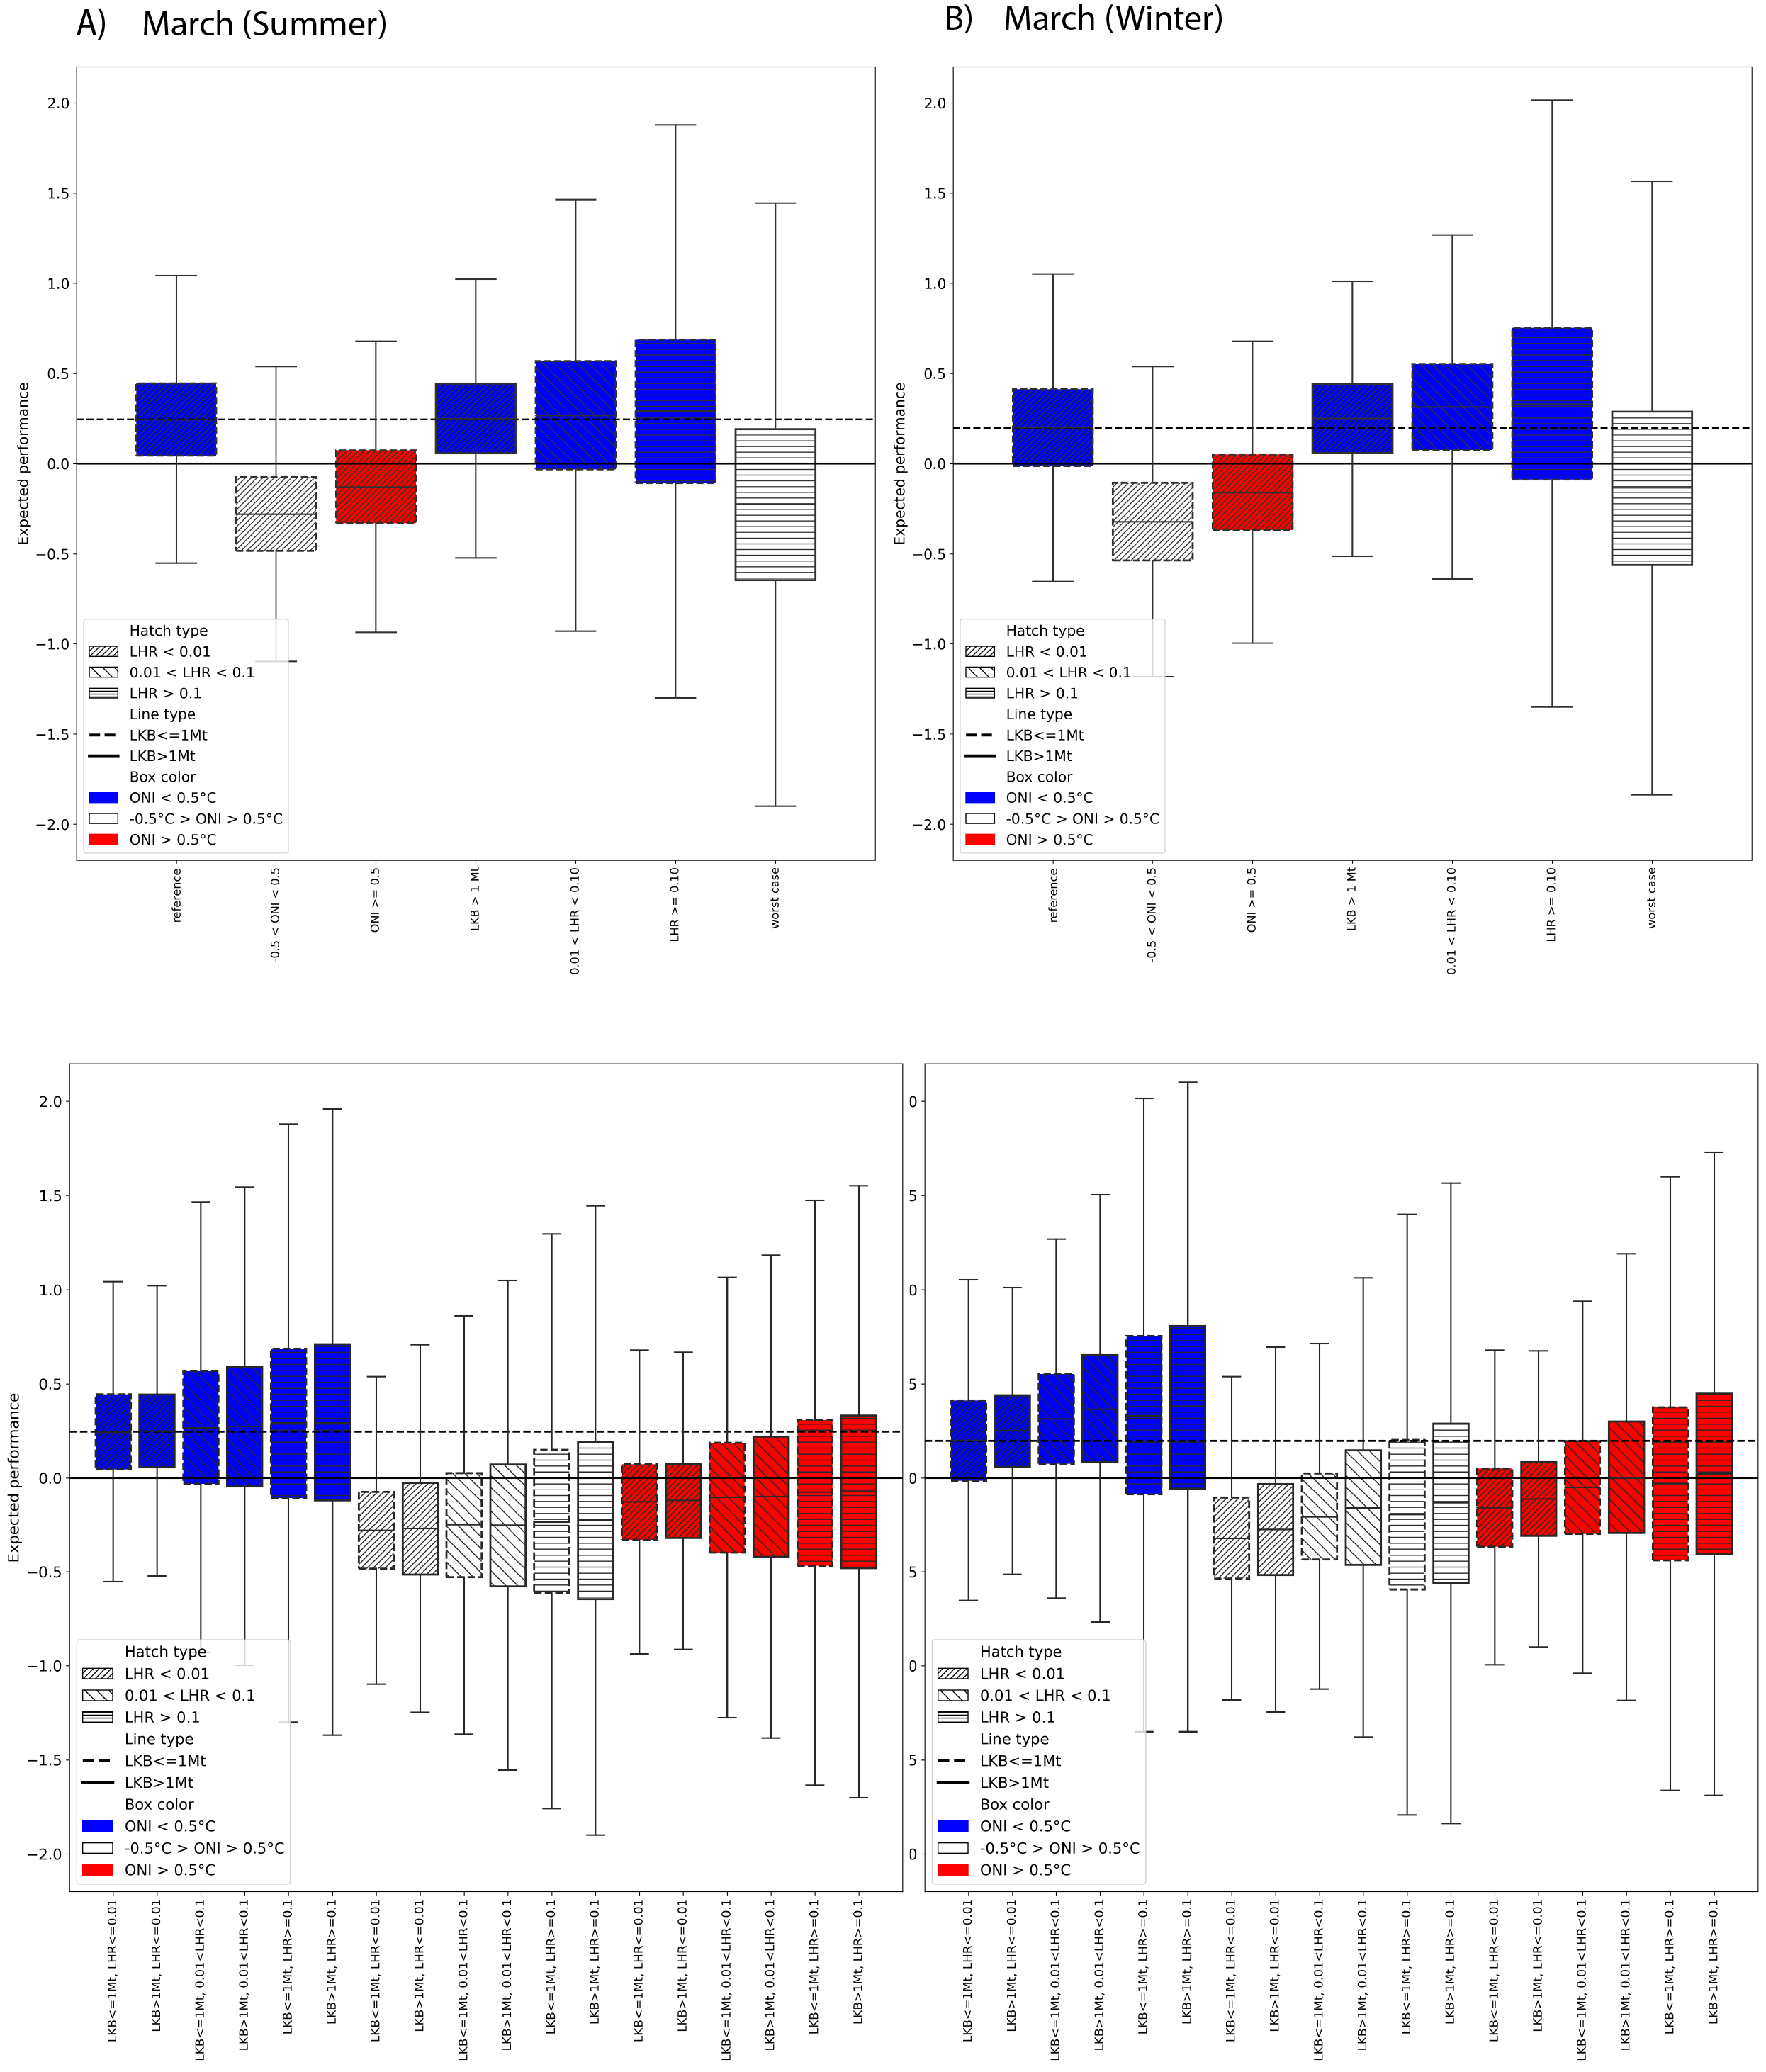
\includegraphics[width=1\linewidth]{./Watters EMM figures/All spp summer then winter 37} \hfill{}

\caption{Model output for the alternatve Watters et al. 2020 scenario outlined above (all species initially present, Adélie and Chinstrap penguins migrate out of the area after breeding, LKB and LHR rescaled to SSMU and March included in summer or winter).   Selected cases as per Watters et al. 2020 for March in A) Summer and B) Winter are provided, with the corresponding case-by-case boxplots presented beneath.  Boxplots are colour-coded by ONI state (red=warm, white=neutral, blue=cold).  In all cases, the marginal effect of ONI dominated the expected performance of penguins against their long-term mean, irrespective of LKB or LHR.}\label{fig:Scenario plot 1}
\end{figure}

\begin{figure}

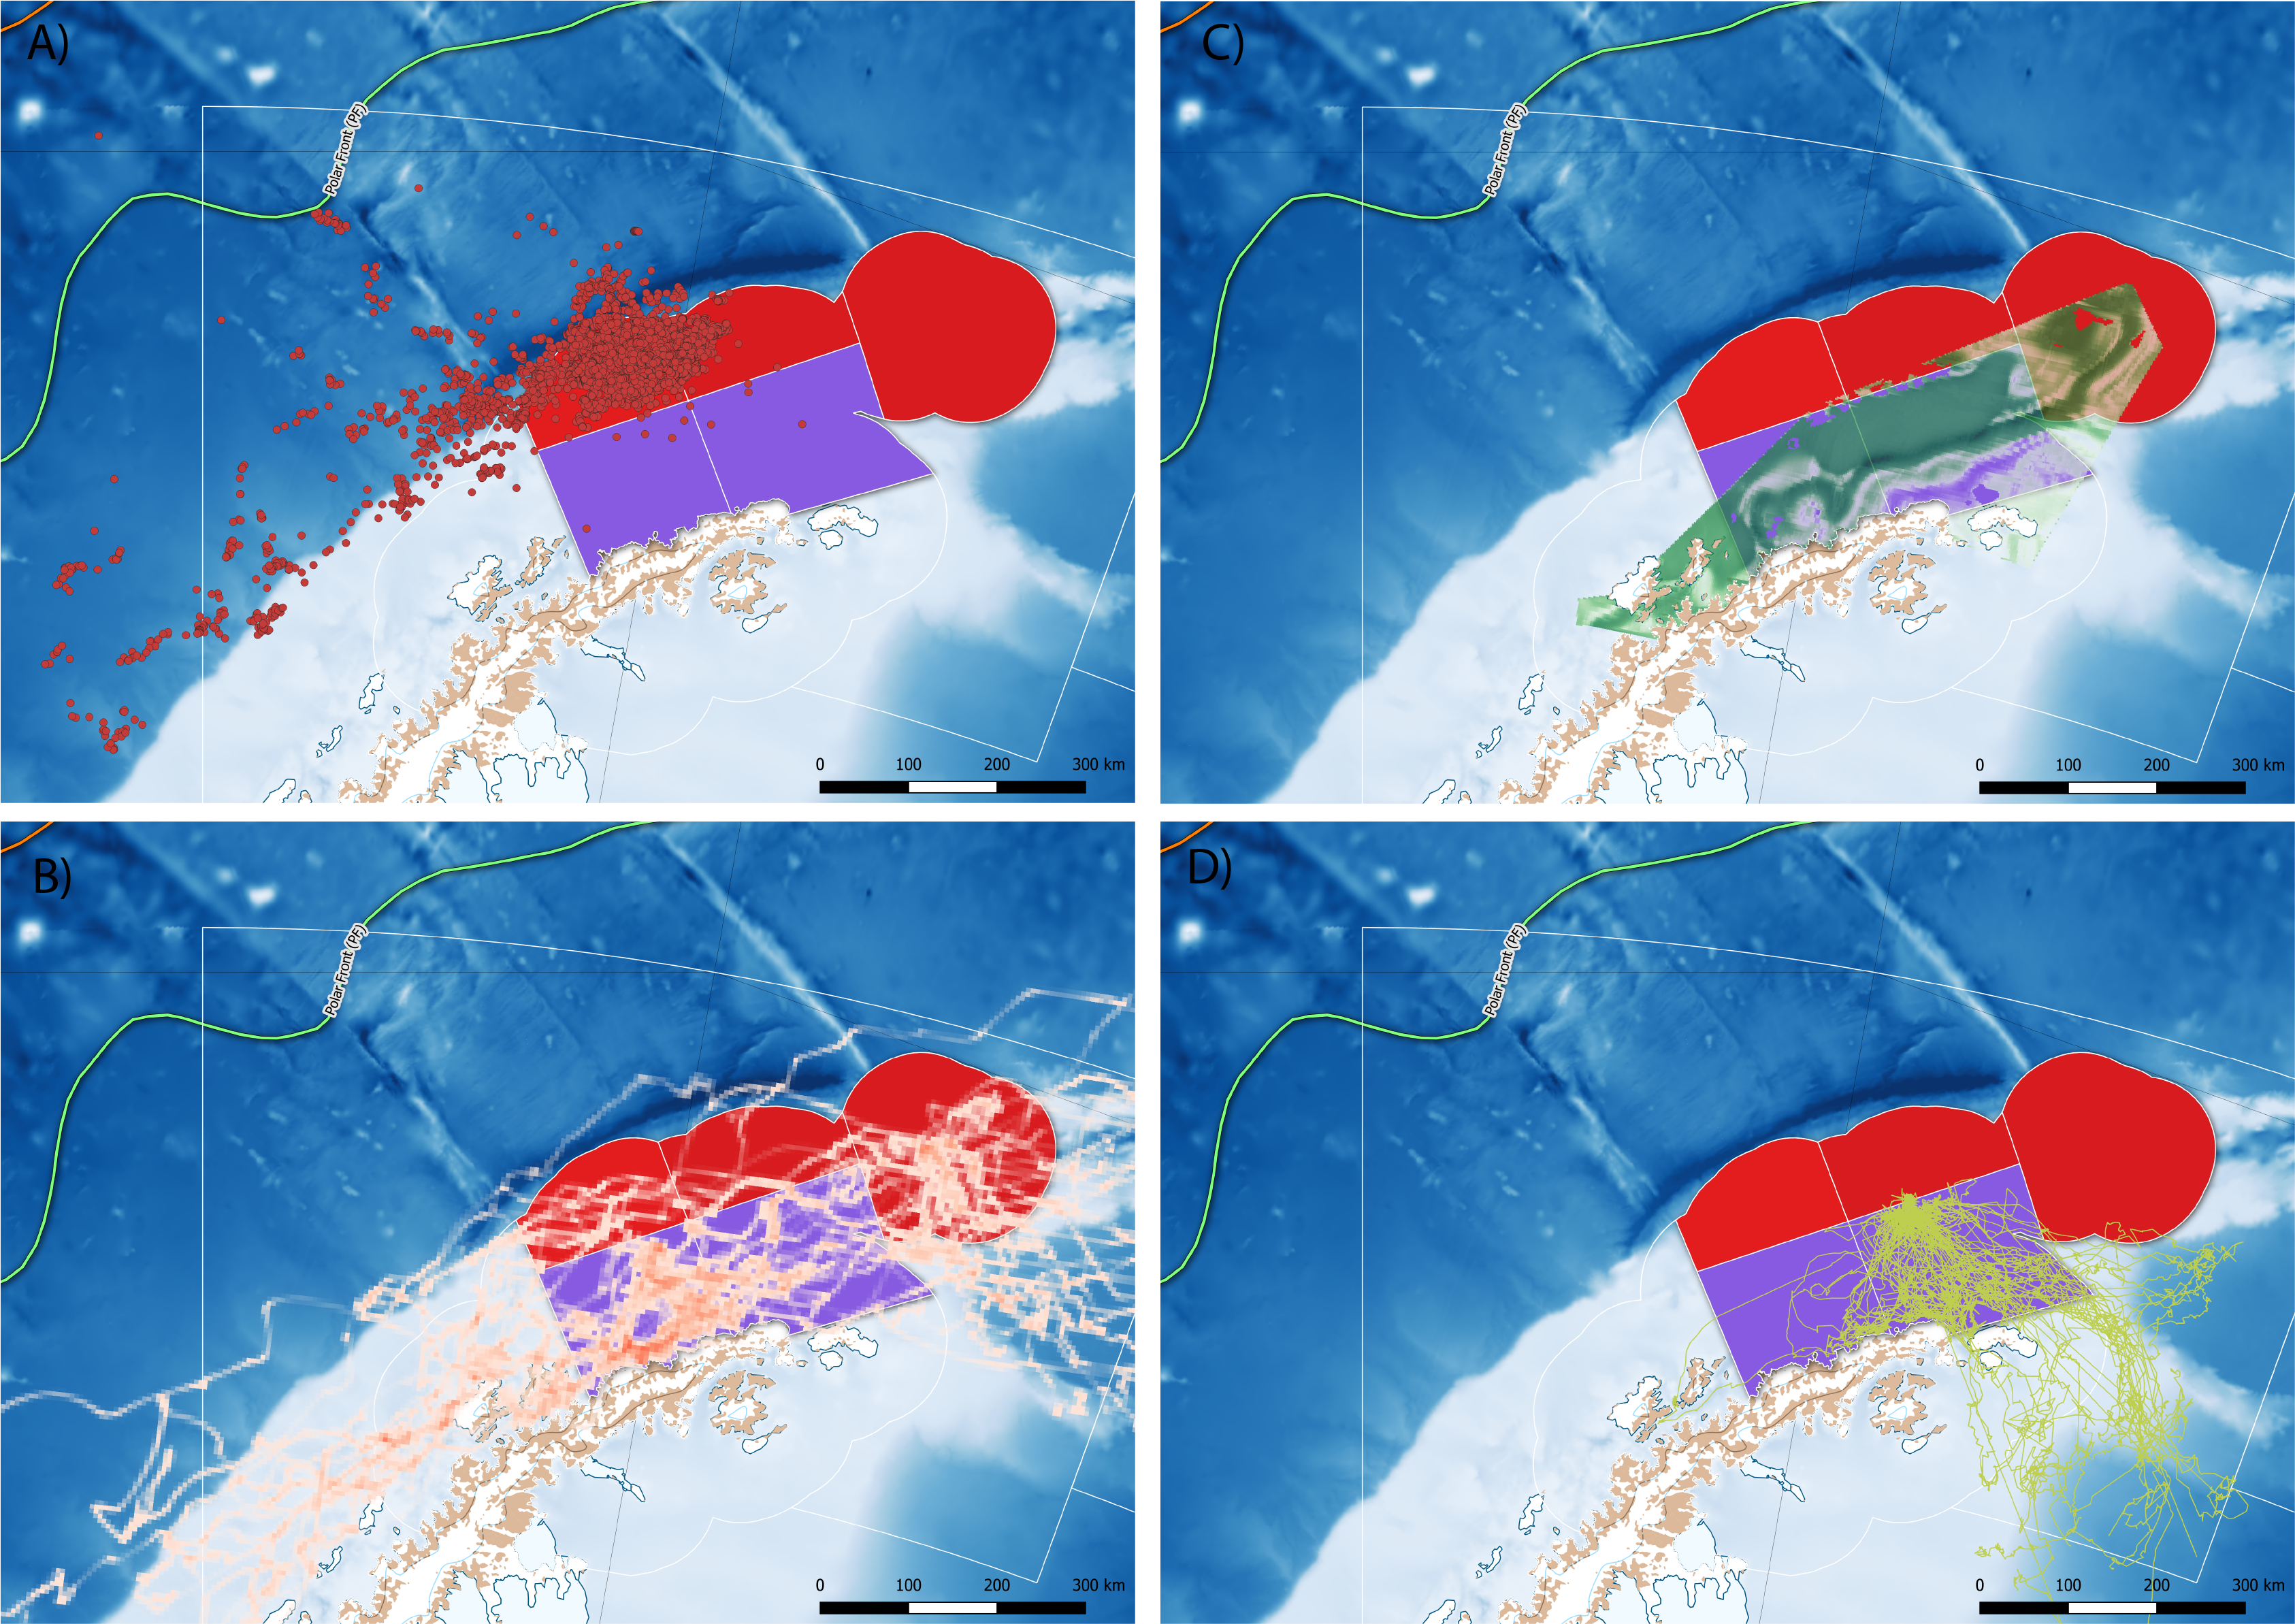
\includegraphics[width=1\linewidth]{./Watters EMM figures/Other spp distribution} \hfill{}

\caption{The summer distribution of foraging effort by A) adult female Antarctic fur seals (adapted from telemetry data available in Hinke et al. 2017), B) migratory adult male Antarctic fur seals (adapted from Lowther et al. 2020) C) humpback whales throughout December (adapted from Johannessen et al., this meeting) and D) nonbreeding adult Adélie penguins during the breeding season (adapted from data in Oosthuizen et al., this meeting). Potential effects of competitive overlap between pygoscelid penguins and other krill dependent predators, particularly those who have increased their abundance dramatically over the preceding 40 years, are excluded from both approaches, creating an unrealistic set of boundary conditions for interpreting the variance in penguin vital rates.}\label{fig:other species plots}
\end{figure}

\begin{figure}
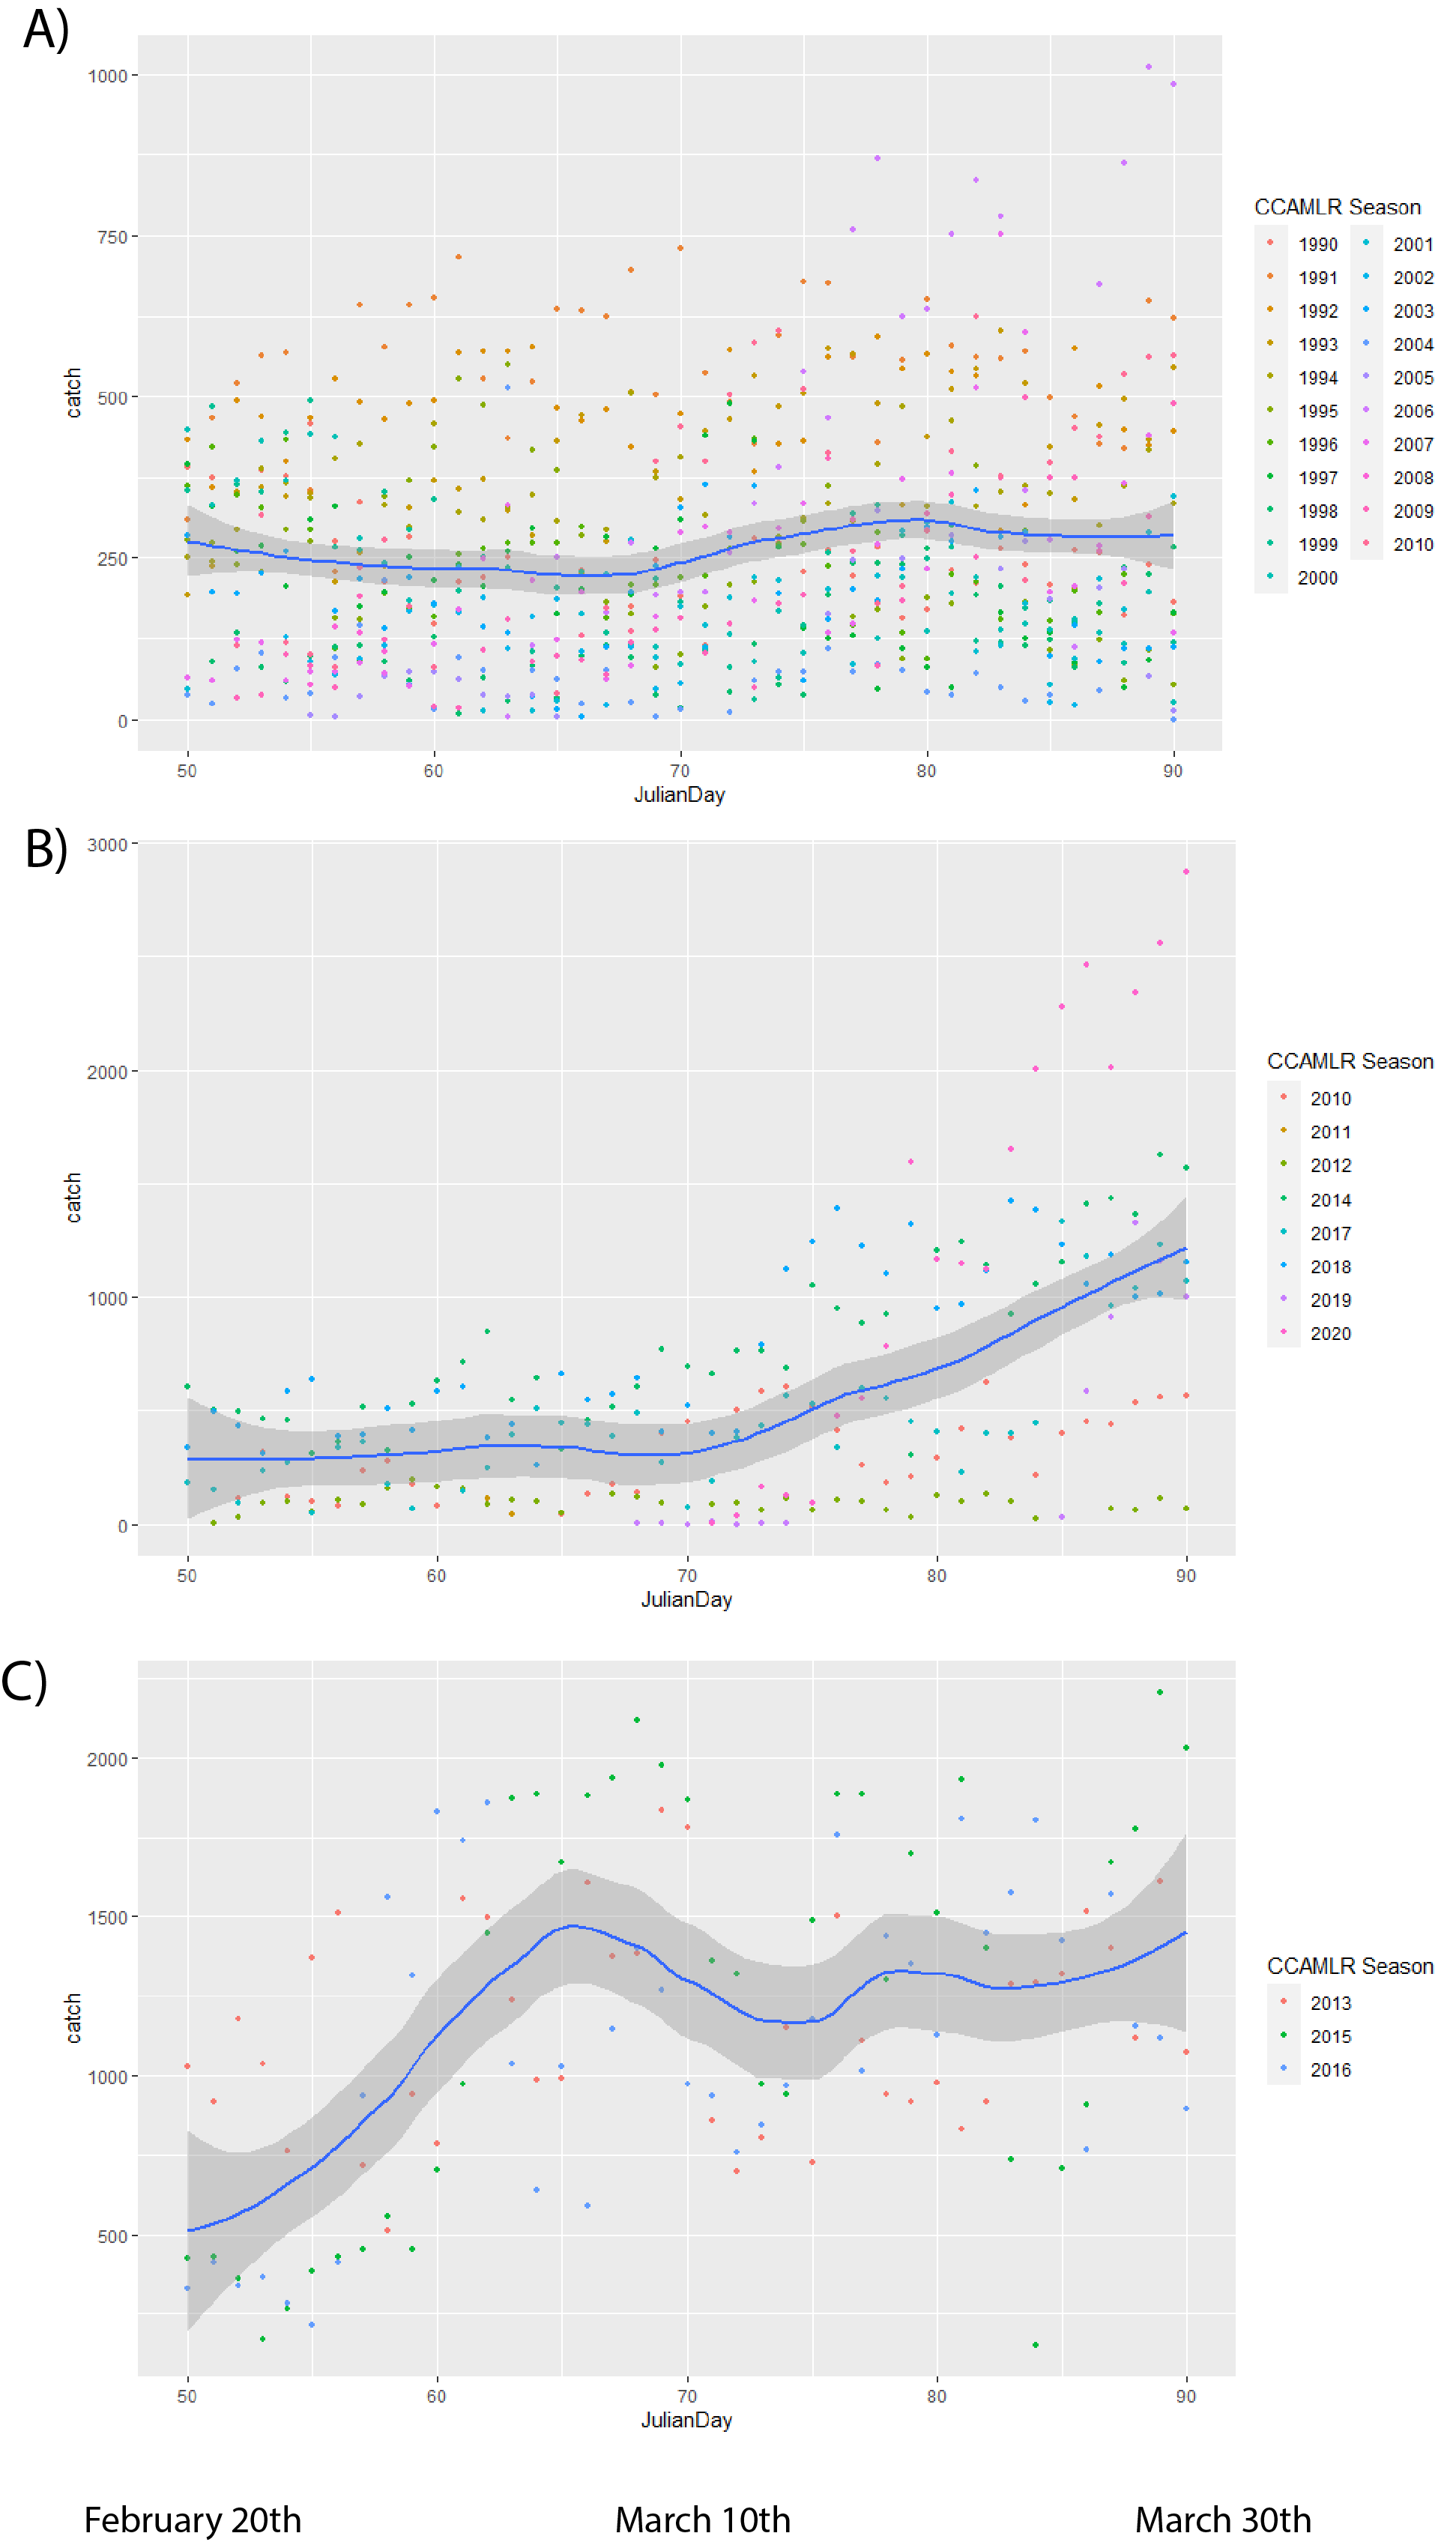
\includegraphics[width=0.6\linewidth]{./Watters EMM figures/catch march 481} \caption{Daily accumulated catch (and fitted LOESS smooth curves) in Subarea 48.1 between 20$^{th}$ February and March 31$^{st}$ between A) 1990-2010 and B) 2010 to 2020. Catch in the Subarea was relatively consistent during the latter stages of penguin breeding at approximately 250tonnes/d (NOTE: different scaling of catch on y-axis between plots).  However, since 2010 there has been a tendency for the fishery to increase its effort in the Subarea, starting around the middle of March. C) During this latter period, the fishery increased effort earlier on three occasions (2013, 2015 and 2016), starting before the beginning of March.}\label{fig:March Subarea 48.1 fishing plot}
\end{figure}
\blandscape

\begin{longtable}[t]{lccccc}
\caption{\label{tab:Table 1 Scenario Original}Original table in Watters et al. 2020.  In this and all subsequent tables below, the posterior and posterior predictive probabilities that the expected performance of penguins given the effects in the left hand column are less than the expected performance given the drivers in the column headings are provided. Worst Case is represented by neutral ONI; LHR  $\geqslant$ 0.1; and LKB $\geqslant$ 1Mt.  The Best Case is represented by La Niña conditions, low LKB and low LHR.}\\
\toprule
Effects & Best Case & -0.5 $^\circ$ C < ONI < +0.5 $^\circ$ C & ONI $\geqslant+0.5$ & Long-term $\mu$ & Long-term predicted $\mu$\\
\midrule
Best case & \- & \- & \- & 0.04 & 0.36\\
ONI Neutral & 1.00 & \- & \- & 0.89 & 0.59\\
ONI warm & 0.99 & \- & \- & 0.52 & 0.51\\
LKB High & 0.71 & 0.02 & 0.12 & 0.01 & 0.41\\
LHR medium & 0.75 & 0.16 & 0.31 & 0.32 & 0.44\\
\addlinespace
LHR high & 0.93 & 0.39 & 0.60 & 0.64 & 0.54\\
Worst case & 0.99 & \- & \- & 0.99 & 0.78\\
\bottomrule
\end{longtable}

\begin{longtable}[t]{lccccc}
\caption{\label{tab:Table 1 Scenario 37a}Posterior and posterior predictive probabilities extracted from the model output for alternatve Watters et al. 2020 scenario outlined above with March attributed to winter (Adélie and Chinstrap penguins migrate out of the area after breeding, LKB and LHR rescaled to SSMU). Under this scenario, performance against the long term mean is worst for neutral and warm ONI conditions.}\\
\toprule
Effects & Best Case & -0.5 $^\circ$ C < ONI < +0.5 $^\circ$ C & ONI $\geqslant+0.5$ & Long-term $\mu$ & Long-term predicted $\mu$\\
\midrule
Best case & \- & \- & \- & 0.04 & 0.40\\
ONI Neutral & 1.00 & \- & \- & 0.97 & 0.62\\
ONI warm & 0.99 & \- & \- & 0.81 & 0.56\\
LKB High & 0.49 & 0.01 & 0.05 & 0.03 & 0.40\\
LHR medium & 0.46 & 0.04 & 0.09 & 0.14 & 0.39\\
\addlinespace
LHR high & 0.45 & 0.10 & 0.16 & 0.23 & 0.39\\
Worst case & 0.84 & \- & \- & 0.71 & 0.59\\
\bottomrule
\end{longtable}
\elandscape
\blandscape

\begin{longtable}[t]{lccccc}
\caption{\label{tab:Table 1 Scenario 37b}Posterior and posterior predictive probabilities extracted from the model output for alternatve Watters et al. 2020 scenario outlined above with March attributed to summer (Adélie and Chinstrap penguins migrate out of the area after breeding, LKB and LHR rescaled to SSMU). Under this scenario performance against the long term mean is also worst for neutral and warm ONI conditions.}\\
\toprule
Effects & Best Case & -0.5 $^\circ$ C < ONI < +0.5 $^\circ$ C & ONI $\geqslant+0.5$ & Long-term $\mu$ & Long-term predicted $\mu$\\
\midrule
Best case & \- & \- & \- & 0.10 & 0.42\\
ONI Neutral & 1.00 & \- & \- & 0.98 & 0.63\\
ONI warm & 0.99 & \- & \- & 0.86 & 0.56\\
LKB High & 0.40 & 0.00 & 0.04 & 0.03 & 0.40\\
LHR medium & 0.27 & 0.01 & 0.02 & 0.04 & 0.37\\
\addlinespace
LHR high & 0.37 & 0.08 & 0.13 & 0.21 & 0.38\\
Worst case & 0.76 & \- & \- & 0.63 & 0.55\\
\bottomrule
\end{longtable}

\elandscape
\blandscape

\elandscape
\blandscape

\elandscape

\begin{longtable}[]{@{}ccc@{}}
\caption{Frequency distribution (percent) of intervals between
consecutive breeding surveys for chinstrap and gentoo penguins used by
Kruger et al 2021.}\tabularnewline
\toprule
\begin{minipage}[b]{0.20\columnwidth}\centering
~\strut
\end{minipage} & \begin{minipage}[b]{0.15\columnwidth}\centering
Chinstrap\strut
\end{minipage} & \begin{minipage}[b]{0.11\columnwidth}\centering
Gentoo\strut
\end{minipage}\tabularnewline
\midrule
\endfirsthead
\toprule
\begin{minipage}[b]{0.20\columnwidth}\centering
~\strut
\end{minipage} & \begin{minipage}[b]{0.15\columnwidth}\centering
Chinstrap\strut
\end{minipage} & \begin{minipage}[b]{0.11\columnwidth}\centering
Gentoo\strut
\end{minipage}\tabularnewline
\midrule
\endhead
\begin{minipage}[t]{0.20\columnwidth}\centering
\textbf{1 year}\strut
\end{minipage} & \begin{minipage}[t]{0.15\columnwidth}\centering
63.11\strut
\end{minipage} & \begin{minipage}[t]{0.11\columnwidth}\centering
69.19\strut
\end{minipage}\tabularnewline
\begin{minipage}[t]{0.20\columnwidth}\centering
\textbf{\textgreater1 year}\strut
\end{minipage} & \begin{minipage}[t]{0.15\columnwidth}\centering
26.16\strut
\end{minipage} & \begin{minipage}[t]{0.11\columnwidth}\centering
47.05\strut
\end{minipage}\tabularnewline
\begin{minipage}[t]{0.20\columnwidth}\centering
\textbf{\textgreater2 years}\strut
\end{minipage} & \begin{minipage}[t]{0.15\columnwidth}\centering
15.26\strut
\end{minipage} & \begin{minipage}[t]{0.11\columnwidth}\centering
14.26\strut
\end{minipage}\tabularnewline
\begin{minipage}[t]{0.20\columnwidth}\centering
\textbf{\textgreater3 years}\strut
\end{minipage} & \begin{minipage}[t]{0.15\columnwidth}\centering
8.7\strut
\end{minipage} & \begin{minipage}[t]{0.11\columnwidth}\centering
9.05\strut
\end{minipage}\tabularnewline
\begin{minipage}[t]{0.20\columnwidth}\centering
\textbf{\textgreater4 years}\strut
\end{minipage} & \begin{minipage}[t]{0.15\columnwidth}\centering
6.8\strut
\end{minipage} & \begin{minipage}[t]{0.11\columnwidth}\centering
4.13\strut
\end{minipage}\tabularnewline
\begin{minipage}[t]{0.20\columnwidth}\centering
\textbf{\textgreater5 years}\strut
\end{minipage} & \begin{minipage}[t]{0.15\columnwidth}\centering
3.52\strut
\end{minipage} & \begin{minipage}[t]{0.11\columnwidth}\centering
3.18\strut
\end{minipage}\tabularnewline
\begin{minipage}[t]{0.20\columnwidth}\centering
\textbf{\textgreater6 years}\strut
\end{minipage} & \begin{minipage}[t]{0.15\columnwidth}\centering
3.05\strut
\end{minipage} & \begin{minipage}[t]{0.11\columnwidth}\centering
2.36\strut
\end{minipage}\tabularnewline
\begin{minipage}[t]{0.20\columnwidth}\centering
\textbf{\textgreater7 years}\strut
\end{minipage} & \begin{minipage}[t]{0.15\columnwidth}\centering
2.23\strut
\end{minipage} & \begin{minipage}[t]{0.11\columnwidth}\centering
0.94\strut
\end{minipage}\tabularnewline
\begin{minipage}[t]{0.20\columnwidth}\centering
\textbf{\textgreater8 years}\strut
\end{minipage} & \begin{minipage}[t]{0.15\columnwidth}\centering
1.76\strut
\end{minipage} & \begin{minipage}[t]{0.11\columnwidth}\centering
0.94\strut
\end{minipage}\tabularnewline
\begin{minipage}[t]{0.20\columnwidth}\centering
\textbf{\textgreater9 years}\strut
\end{minipage} & \begin{minipage}[t]{0.15\columnwidth}\centering
1.76\strut
\end{minipage} & \begin{minipage}[t]{0.11\columnwidth}\centering
0.47\strut
\end{minipage}\tabularnewline
\begin{minipage}[t]{0.20\columnwidth}\centering
\textbf{\textgreater14 years}\strut
\end{minipage} & \begin{minipage}[t]{0.15\columnwidth}\centering
1.29\strut
\end{minipage} & \begin{minipage}[t]{0.11\columnwidth}\centering
0.47\strut
\end{minipage}\tabularnewline
\begin{minipage}[t]{0.20\columnwidth}\centering
\textbf{\textgreater15 years}\strut
\end{minipage} & \begin{minipage}[t]{0.15\columnwidth}\centering
1.29\strut
\end{minipage} & \begin{minipage}[t]{0.11\columnwidth}\centering
0\strut
\end{minipage}\tabularnewline
\begin{minipage}[t]{0.20\columnwidth}\centering
\textbf{\textgreater19 years}\strut
\end{minipage} & \begin{minipage}[t]{0.15\columnwidth}\centering
0.82\strut
\end{minipage} & \begin{minipage}[t]{0.11\columnwidth}\centering
0\strut
\end{minipage}\tabularnewline
\bottomrule
\end{longtable}

\newpage
\blandscape
\beginsupplement

\hypertarget{supplementary-material}{%
\section{Supplementary material}\label{supplementary-material}}

\begin{figure}
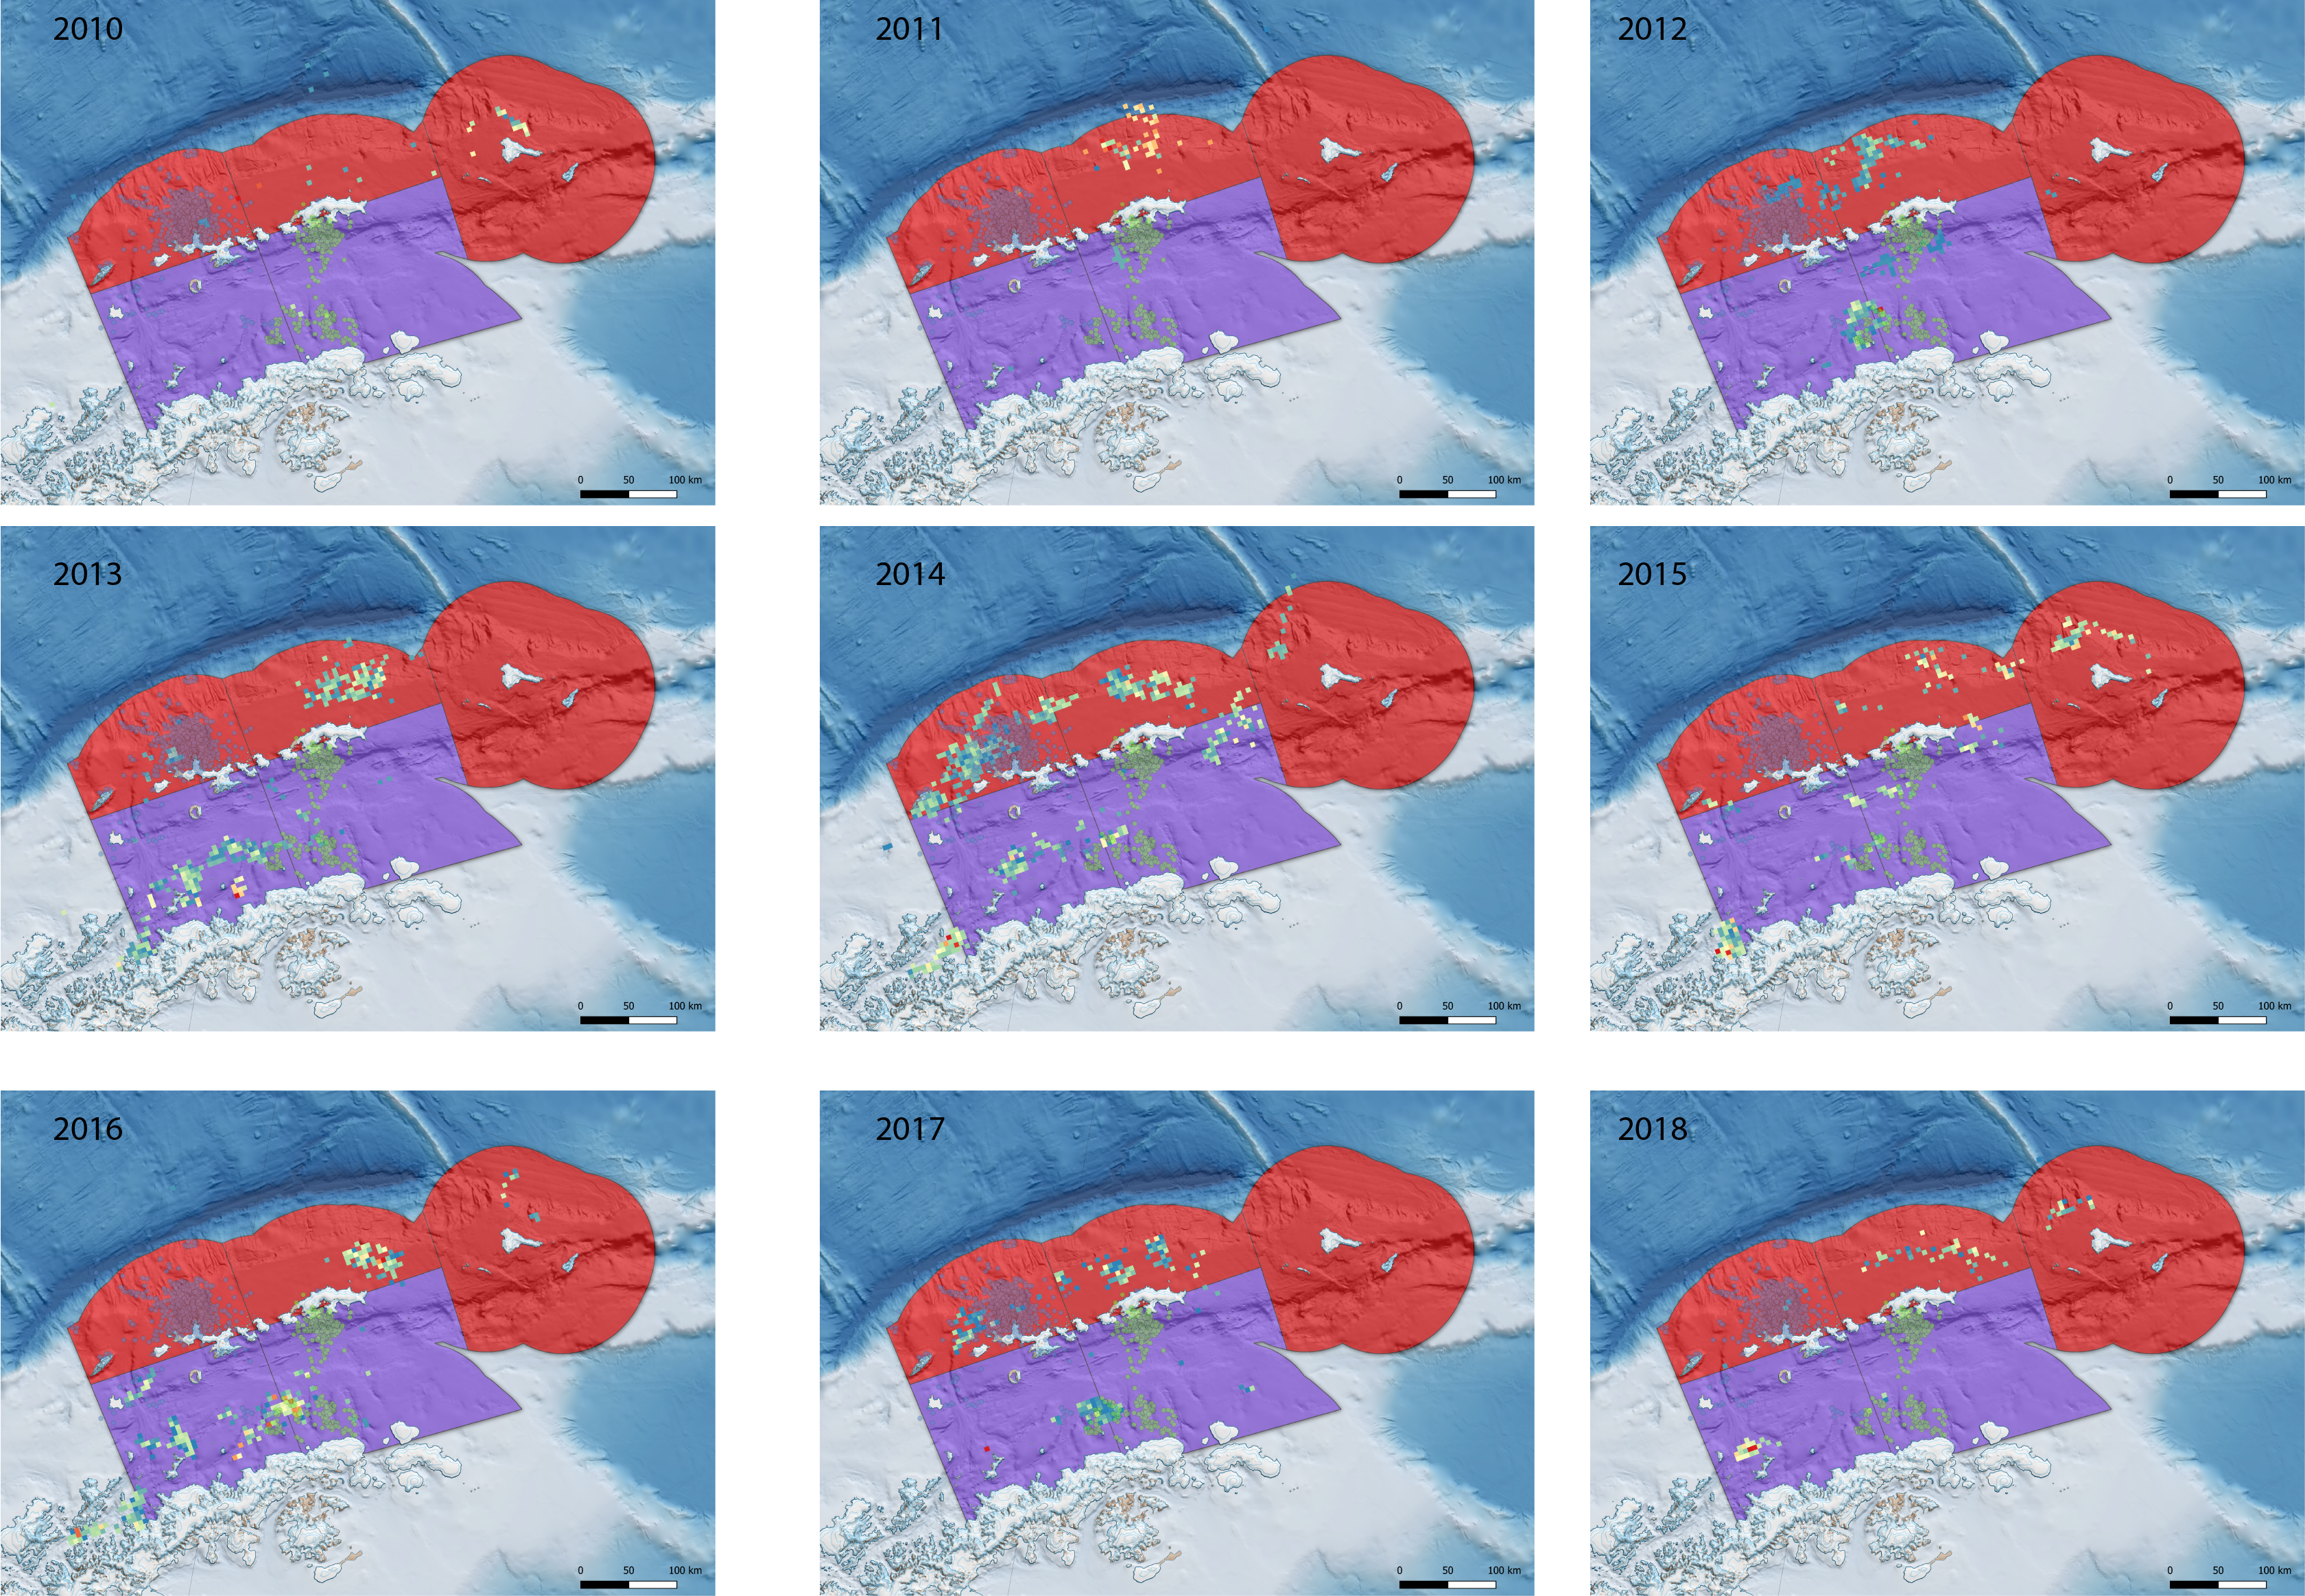
\includegraphics[width=0.8\linewidth]{./Watters EMM figures/summer catch/Year by year catch} \caption{C1 Catch and Effort data for 2010 - 2018, for all catches during the period of the austral summer relating to Adélie and Chinstrap penguins in Subarea 48.1 (i.e. up to $10^{th}$ March).  The telemetry data presented in Hinke et al. 2017 for Chinstrap penguins at both Cape Shireff and Copacabana and the gSSMU used in the Watters et al. 2020 paper are superimposed to highlight the extreme variability in actual catch, relative to the scale of LHR used to reflect interactions with penguins.  Our reanalysis re-scaled LHR to the SSMU level, though we contend that for the purposes of matching predator data at appropriate spatial scales even this is too coarse a resolution.}\label{fig:Supplementary Figure 1}
\end{figure}
\elandscape
\newpage

\hypertarget{citations}{%
\section*{Citations}\label{citations}}
\addcontentsline{toc}{section}{Citations}

\hypertarget{refs}{}
\leavevmode\hypertarget{ref-Black2016}{}%
Black, C.E., 2016. A comprehensive review of the phenology of Pygoscelis
penguins. Polar Biology 39, 405--432.
doi:\href{https://doi.org/10.1007/s00300-015-1807-8}{10.1007/s00300-015-1807-8}

\leavevmode\hypertarget{ref-capotondiUnderstandingENSODiversity2015}{}%
Capotondi, A., Wittenberg, A.T., Newman, M., Di Lorenzo, E., Yu, J.-Y.,
Braconnot, P., Cole, J., Dewitte, B., Giese, B., Guilyardi, E., 2015.
Understanding ENSO diversity. Bulletin of the American Meteorological
Society 96, 921--938.

\leavevmode\hypertarget{ref-Clem2016}{}%
Clem, K.R., Renwick, J.A., McGregor, J., Fogt, R.L., 2016. The relative
influence of ENSO and SAM on antarctic Peninsula climate. Journal of
Geophysical Research 121, 9324--9341.
doi:\href{https://doi.org/10.1002/2016JD025305}{10.1002/2016JD025305}

\leavevmode\hypertarget{ref-doddridgeModulationSeasonalCycle2017}{}%
Doddridge, E.W., Marshall, J., 2017. Modulation of the seasonal cycle of
Antarctic sea ice extent related to the Southern Annular Mode.
Geophysical Research Letters 44, 9761--9768.

\leavevmode\hypertarget{ref-Hinke2017}{}%
Hinke, J.T., Cossio, A.M., Goebel, M.E., Reiss, C.S., Trivelpiece, W.Z.,
Watters, G.M., 2017. Identifying Risk: Concurrent overlap of the
antarctic krill fishery with krill-dependent predators in the scotia
sea. PLoS ONE 12, e0170132.
doi:\href{https://doi.org/10.1371/journal.pone.0170132}{10.1371/journal.pone.0170132}

\leavevmode\hypertarget{ref-Hinke2015}{}%
Hinke, J.T., Polito, M.J., Goebel, M.E., Jarvis, S., Reiss, C.S.,
Thorrold, S.R., Trivelpiece, W.Z., Watters, G.M., 2015. Spatial and
isotopic niche partitioning during winter in chinstrap and Adélie
penguins from the South Shetland Islands. Ecosphere 6, 125.
doi:\href{https://doi.org/10.1890/ES14-00287.1}{10.1890/ES14-00287.1}

\leavevmode\hypertarget{ref-Hinke2019}{}%
Hinke, J.T., Santos, M.M., Korczak-Abshire, M., Milinevsky, G., Watters,
G.M., 2019. Individual variation in migratory movements of chinstrap
penguins leads to widespread occupancy of ice-free winter habitats over
the continental shelf and deep ocean basins of the Southern Ocean. PLoS
ONE 14.
doi:\href{https://doi.org/10.1371/journal.pone.0226207}{10.1371/journal.pone.0226207}

\leavevmode\hypertarget{ref-Humphries2017}{}%
Humphries, G.R.W., Naveen, R., Schwaller, M., Che-Castaldo, C.,
McDowall, P., Schrimpf, M., Lynch, H.J., 2017. Mapping Application for
Penguin Populations and Projected Dynamics (MAPPPD): Data and tools for
dynamic management and decision support. Polar Record 53, 160--166.
doi:\href{https://doi.org/10.1017/S0032247417000055}{10.1017/S0032247417000055}

\leavevmode\hypertarget{ref-korczak-abshireCoastalRegionsNorthern2021}{}%
Korczak-Abshire, M., Hinke, J.T., Milinevsky, G., Juáres, M.A., Watters,
G.M., 2021. Coastal regions of the northern Antarctic Peninsula are key
for gentoo populations. Biology letters 17, 20200708.

\leavevmode\hypertarget{ref-Kruger2021}{}%
Krüger, L., Huerta, M.F., Santa Cruz, F., Cárdenas, C.A., 2021.
Antarctic krill fishery effects over penguin populations under adverse
climate conditions: Implications for the management of fishing
practices. Ambio 50, 560--571.
doi:\href{https://doi.org/10.1007/s13280-020-01386-w}{10.1007/s13280-020-01386-w}

\leavevmode\hypertarget{ref-kwokSpatialPatternsVariability2002}{}%
Kwok, R., Comiso, J.C., 2002. Spatial patterns of variability in
Antarctic surface temperature: Connections to the Southern Hemisphere
Annular Mode and the Southern Oscillation. Geophysical Research Letters
29, 50--1.

\leavevmode\hypertarget{ref-Lowther2020}{}%
Lowther, A.D., Staniland, I., Lydersen, C., Kovacs, K.M., 2020. Male
Antarctic fur seals: Neglected food competitors of bioindicator species
in the context of an increasing Antarctic krill fishery. Scientific
Reports 10.
doi:\href{https://doi.org/10.1038/s41598-020-75148-9}{10.1038/s41598-020-75148-9}

\leavevmode\hypertarget{ref-santoraKrillSpaceComparative2012}{}%
Santora, J.A., Sydeman, W.J., Schroeder, I.D., Reiss, C.S., Wells, B.K.,
Field, J.C., Cossio, A.M., Loeb, V.J., 2012. Krill space: A comparative
assessment of mesoscale structuring in polar and temperate marine
ecosystems. ICES Journal of Marine Science 69, 1317--1327.

\leavevmode\hypertarget{ref-Santora2013}{}%
Santora, J.A., Veit, R.R., 2013. Spatio-temporal persistence of top
predator hotspots near the Antarctic Peninsula. Marine Ecology Progress
Series 487, 287--304.
doi:\href{https://doi.org/10.3354/meps10350}{10.3354/meps10350}

\leavevmode\hypertarget{ref-Warwick-Evans2018}{}%
Warwick-Evans, V., Ratcliffe, N., Lowther, A.D., Manco, F., Ireland, L.,
Clewlow, H.L., Trathan, P.N., 2018. Using habitat models for chinstrap
penguins Pygoscelis antarctica to advise krill fisheries management
during the penguin breeding season. Diversity and Distributions 24,
1756--1771.
doi:\href{https://doi.org/10.1111/ddi.12817}{10.1111/ddi.12817}

\leavevmode\hypertarget{ref-Watters2020}{}%
Watters, G.M., Hinke, J.T., Reiss, C.S., 2020. Long-term observations
from Antarctica demonstrate that mismatched scales of fisheries
management and predator-prey interaction lead to erroneous conclusions
about precaution. Scientific Reports 10.
doi:\href{https://doi.org/10.1038/s41598-020-59223-9}{10.1038/s41598-020-59223-9}


\end{document}


